\cleardoublepage
\chapter{Splicing signatures of progressive tau pathology in AD mouse model}\label{ch: transcriptional_global_differences}

\section{Introduction}
There is increasing evidence on the role of transcriptional dysregulation and aberrant splicing in the development and pathogenesis of AD (described in \cref{intro:AD_alteredsplicing}). Recent transcriptome profiling studies have identified changes in splicing and transcript expression in both human AD post-mortem brain tissue and AD mouse models (reviewed in \cref{tab: AS_ADHuman_studies} and \cref{tab: AS_ADMouse_studies}, respectively). However, to date, these studies have relied on short-read RNA sequencing approaches, which cannot reliably detect specific isoforms (as discussed in \cref{rnaseq_intro}) and have broadly ignored identifying differences at the transcript level. In contrast, we have illustrated the power of long-read sequencing to identify full-length transcripts and improve our annotations of alternatively-spliced isoforms in the cortex of the rTg4510 mouse model of AD tauopathy (\cref{ch: whole_transcriptome}). 

While long-read sequencing approaches are currently considered to be only semi-quantitative, recent studies have delivered promising strategies for transcript-based analysis by using a hybrid approach\cite{Tseng2021}: the alignment of short-read RNA-Seq data to improved transcriptome annotations derived from long-read data (as depicted in \cref{fig:isoform_quant_strategy}). This has enabled the identification of differentially expressed isoforms and analysis of differential transcript usage between experimental groups\cite{Tseng2021}. 

Following on from the results presented in \textbf{Chapter 4}, this chapter aimed to exploit the cortical long-read sequencing datasets (hereby referred to as “Iso-Seq global dataset”) generated from rTg4510 transgenic (TG) and wild-type (WT) mice to identify transcriptional and splicing alterations associated with progressive tau pathology. The objectives of this chapter were as follows: 
\begin{enumerate}
	\item To assess global variation in splicing patterns between rTg4510 TG and WT mice.
	\item To perform differential gene expression analysis and validate differences in gene expression associated with tau pathology from previous RNA-Seq studies. 
	\item To perform differential transcript expression analysis to identify differences in transcript expression associated with tau pathology.   
	\item To perform differential transcript usage analysis to identify genes with significant alterations in isoform proportions between rTg4510 TG and WT mice. 
\end{enumerate} 

\newpage
\section{Methods}

\subsection{Datasets}
All analyses presented in this chapter follow on from \cref{ch: whole_transcriptome} and use the same Iso-Seq long-read datasets generated from 12 female mice (n = 6 WT, n = 6 TG, aged 2 and 8 months, \cref{tab:whole_phenotype}). Briefly, RNA was prepared for Iso-Seq library preparation and SMRT sequencing on the PacBio Sequel (\cref{ch4_methods: isoseq_library}), followed by QC and data processing (\cref{ch4_methods: isoseq_data}). Reads from individual samples were processed separately with \textit{IsoSeq3} and merged for transcript collapse using \textit{Cupcake}. High-quality, full-length transcripts from the merged dataset were then aligned to the mouse reference genome (mm10, GENCODE) using \textit{Minimap2} (v2.17) and re-annotated using \textit{SQANTI3} with no splice junction filtering from short-read RNA-Seq data. ISM transcripts with only the 3' fragment matching reference transcript (3' ISM) were considered technical artefacts resulting from 5' degradation and thus removed.  

\subsection{Quantification of human \textit{MAPT} transgene expression}
\label{ch5: hmapt_quant}
As described in \cref{ch2: rtg4510}, rTg4510 mice recapitulate AD tauopathy through the overexpression of the human tau transgene, MAPT\textsuperscript{P301L}. The presence of the human-specific \textit{MAPT} sequence was therefore determined in the Iso-Seq datasets by using the \textit{grep} Unix command, as QC of sample identity. A 2kb region present in the 3' UTR was chosen as the representative human \textit{MAPT} sequence\cite{Castanho2020}.

\subsection{Characterisation of alternative splicing events} 
Alternative splicing events were examined using a range of packages and custom scripts (as described and implemented in \cref{ch4: transcriptome_annotation}), to assess whether there was a difference in splicing patterns associated with progressive tau pathology in the rTg4510 mouse model. 

\subsection{Gene and isoform quantification}
Gene and isoform expression were estimated using two approaches (as described in \cref{sec: gene_isoform_quant_explained}). Briefly, these were: i) the alignment of short-read RNA-Seq reads to the Iso-Seq-derived transcriptome (hybrid approach) using \textit{Kallisto}\cite{Bray2016} (v0.46.0), and ii) the use of normalised Iso-Seq full-length read counts as a proxy for expression. Full-length read counts for each sample were taken from the \textit{read\_stat.txt} file generated using the \textit{collapse\_isoforms\_by\_sam.py} script (\textit{Cupcake}) with the sequencing run ID as identifiers. 

\subsection{Differential expression analysis}
Differential expression analysis was performed using \textit{tappAS} (fully described in \cref{ch3_tappas_explained}). Briefly, \textit{tappAS} filters out lowly-expressed isoforms, normalises read counts using the TMM approach, and implements \textit{maSigPro}\cite{Conesa2006,Nueda2014,Conesa2017} to elucidate the effects of genotype and age with the following model\cite{Conesa2006}: 

\vspace{0.5cm}
\begin{myequation}[h]
\begin{adjustwidth}{1.8em}{1.8em}
Let \textit{i} denote the genotype group (WT - wild-type mice, TG - rTg4510 transgenic mice), \textit{j} the age (2 or 8 months) and \textit{r} the replicate number (assuming that gene or transcript expression is measured in replicated samples).  
\end{adjustwidth}
\begin{align}
	y_{ijr} =  \:&\beta_{0} + \beta_{1}D_{i} \nonumber
	\\ &+ \delta_{0}T_{ijr} + \delta_{1}T_{ijr}D_{ijr}   \nonumber
\end{align}
\begin{adjustwidth}{1.8em}{1.8em}
where
\begin{conditions*}
	y_{ijr} & normalised expression value for each gene or transcript in the situation \newline \textit{ijr} (genotype group \textit{i} at age \textit{j} of replicate \textit{r}) \\
	D  &  dummy binary variable to distinguish between the genotype groups,\newline whereby 0 and 1 refers to reference (WT) and experimental group (TG), respectively \\
	T  &  age at 2, 8 months described using a polynomial model (degree of 1) \\
	\beta_{0}, \delta_{0} & regression coefficients for reference group (WT) relating to the age \\ 
	\beta_{1}, \delta_{1} & regression coefficients for the difference between experimental group \newline (TG) and reference group (WT) at each age  
\end{conditions*}
therefore, if:
\begin{conditions*}
	FDR(\beta_{1}) < 0.05 & significant expression difference between WT \& TG at 2 mos \\ 
	FDR(\delta_{0}) < 0.05 & significant expression difference in WT across 2 and 8 mos \\
\end{conditions*}
\end{adjustwidth}
\captionsetup{width=0.92\textwidth}
\caption[Linear regression model to determine differential gene and transcript expression]%
{\textbf{Linear regression model to determine differential gene and transcript expression}. The model is adapted from \textit{MaSigPro} and implemented as part of \textit{tappAS}. It identifies differences in gene and transcript expression between two groups (WT - wild-type mice, TG - rTg4510 transgenic mice) at different time points (age in months). FDR - False discovery rate. mos - Months.}    
\end{myequation}


\begin{figure}[!htp]
	\centering
	\includegraphics[page=2,trim={0 5cm 0 4cm},scale = 0.45]{Figures/Tg4510_diff_figures.pdf}
	\captionsetup{width=0.95\textwidth}
	\caption[Different conditions modelled for rTg4510 genotype and age effects]%
	{\textbf{Different conditions modelled for rTg4510 genotype and age effects.} Shown is a linear model implemented in \textit{maSigPro} to dissect genotype and age effects using \textbf{Equation 5.1} between two experimental groups (WT - Wild-type/Control, TG - Transgenic/Case) and across two time points (T1, T2). 
	\\\\
	The regression coefficients from \textbf{Equation 5.1} - $\beta_{1}$, $\delta_{0}$, $\delta_{1}$ - refer to the different variables modelled, the significance of which can be used to infer whether there is a genotype, age or interaction effect. The significance is symbolised by the tick and cross, which refers to adjusted \textit{P} (FDR) < 0.05 and > 0.05 respectively. A significant value of $\beta_{1}$ denotes to a statistically significant difference between WT and TG at T1 (genotype effect), $\delta_{0}$ to a difference in WT over time (age effect), and $\delta_{1}$ to a difference between WT and TG across age (interaction effect).}   
	\label{fig:dea_model}
\end{figure}

Under this model, a differentially expressed gene or transcript between WT and TG mice across age was defined by a statistically significant regression coefficient (adjusted \textit{P} < 0.05) and a regression model with R\textsuperscript{2} > 0.5 (i.e. the amount of variance explained by the model) (\cref{fig:dea_model}). 


\clearpage 
\section{Results}
\subsection{PacBio Iso-Seq run performance and sequencing metrics}
No significant difference in sequencing yield was identified between WT and TG mice (n = 12 samples, two-tailed unpaired t-test, t(10) = -0.636, \textit{P} = 0.539, \cref{fig:rTg4510_sequencing_metrics}\textbf{A}), and no significant correlation was observed between run yield and RIN across samples (n = 12 samples, Pearson's correlation, corr = -0.296, df = 10, \textit{P} = 0.350, \cref{fig:rTg4510_sequencing_metrics}\textbf{B}). No significant difference was also observed in the number of reads (\cref{fig:rTg4510_sequencing_metrics}\textbf{C}) and transcripts generated between WT and TG mice (n = 12 samples, two-tailed unpaired t-test, t = -0.005, df = 10, \textit{P} = 0.996, \cref{fig:rTg4510_sequencing_metrics}\textbf{D}) or by age (n = 12 samples, t = -1.58, df = 10, \textit{P} = 0.15). Notably, a similar read profile was attained for all the samples except the first two samples, which were sequenced using an older chemistry and had a relatively lower throughput. Nonetheless, all the samples were successfully sequenced with optimal runs, as indicated by the high throughput and the similar number of full-length, full-length non-chimeric (FLNC) and poly(A) FLNC reads recovered. ERCC alignment and annotations similarly revealed no difference in the number of ERCC control molecules detected between WT and TG (mean number of ERCC controls: WT = 32.4, 35\%; TG = 32.2, 35.22\%). 

\begin{figure}[htp]
	\begin{center}
		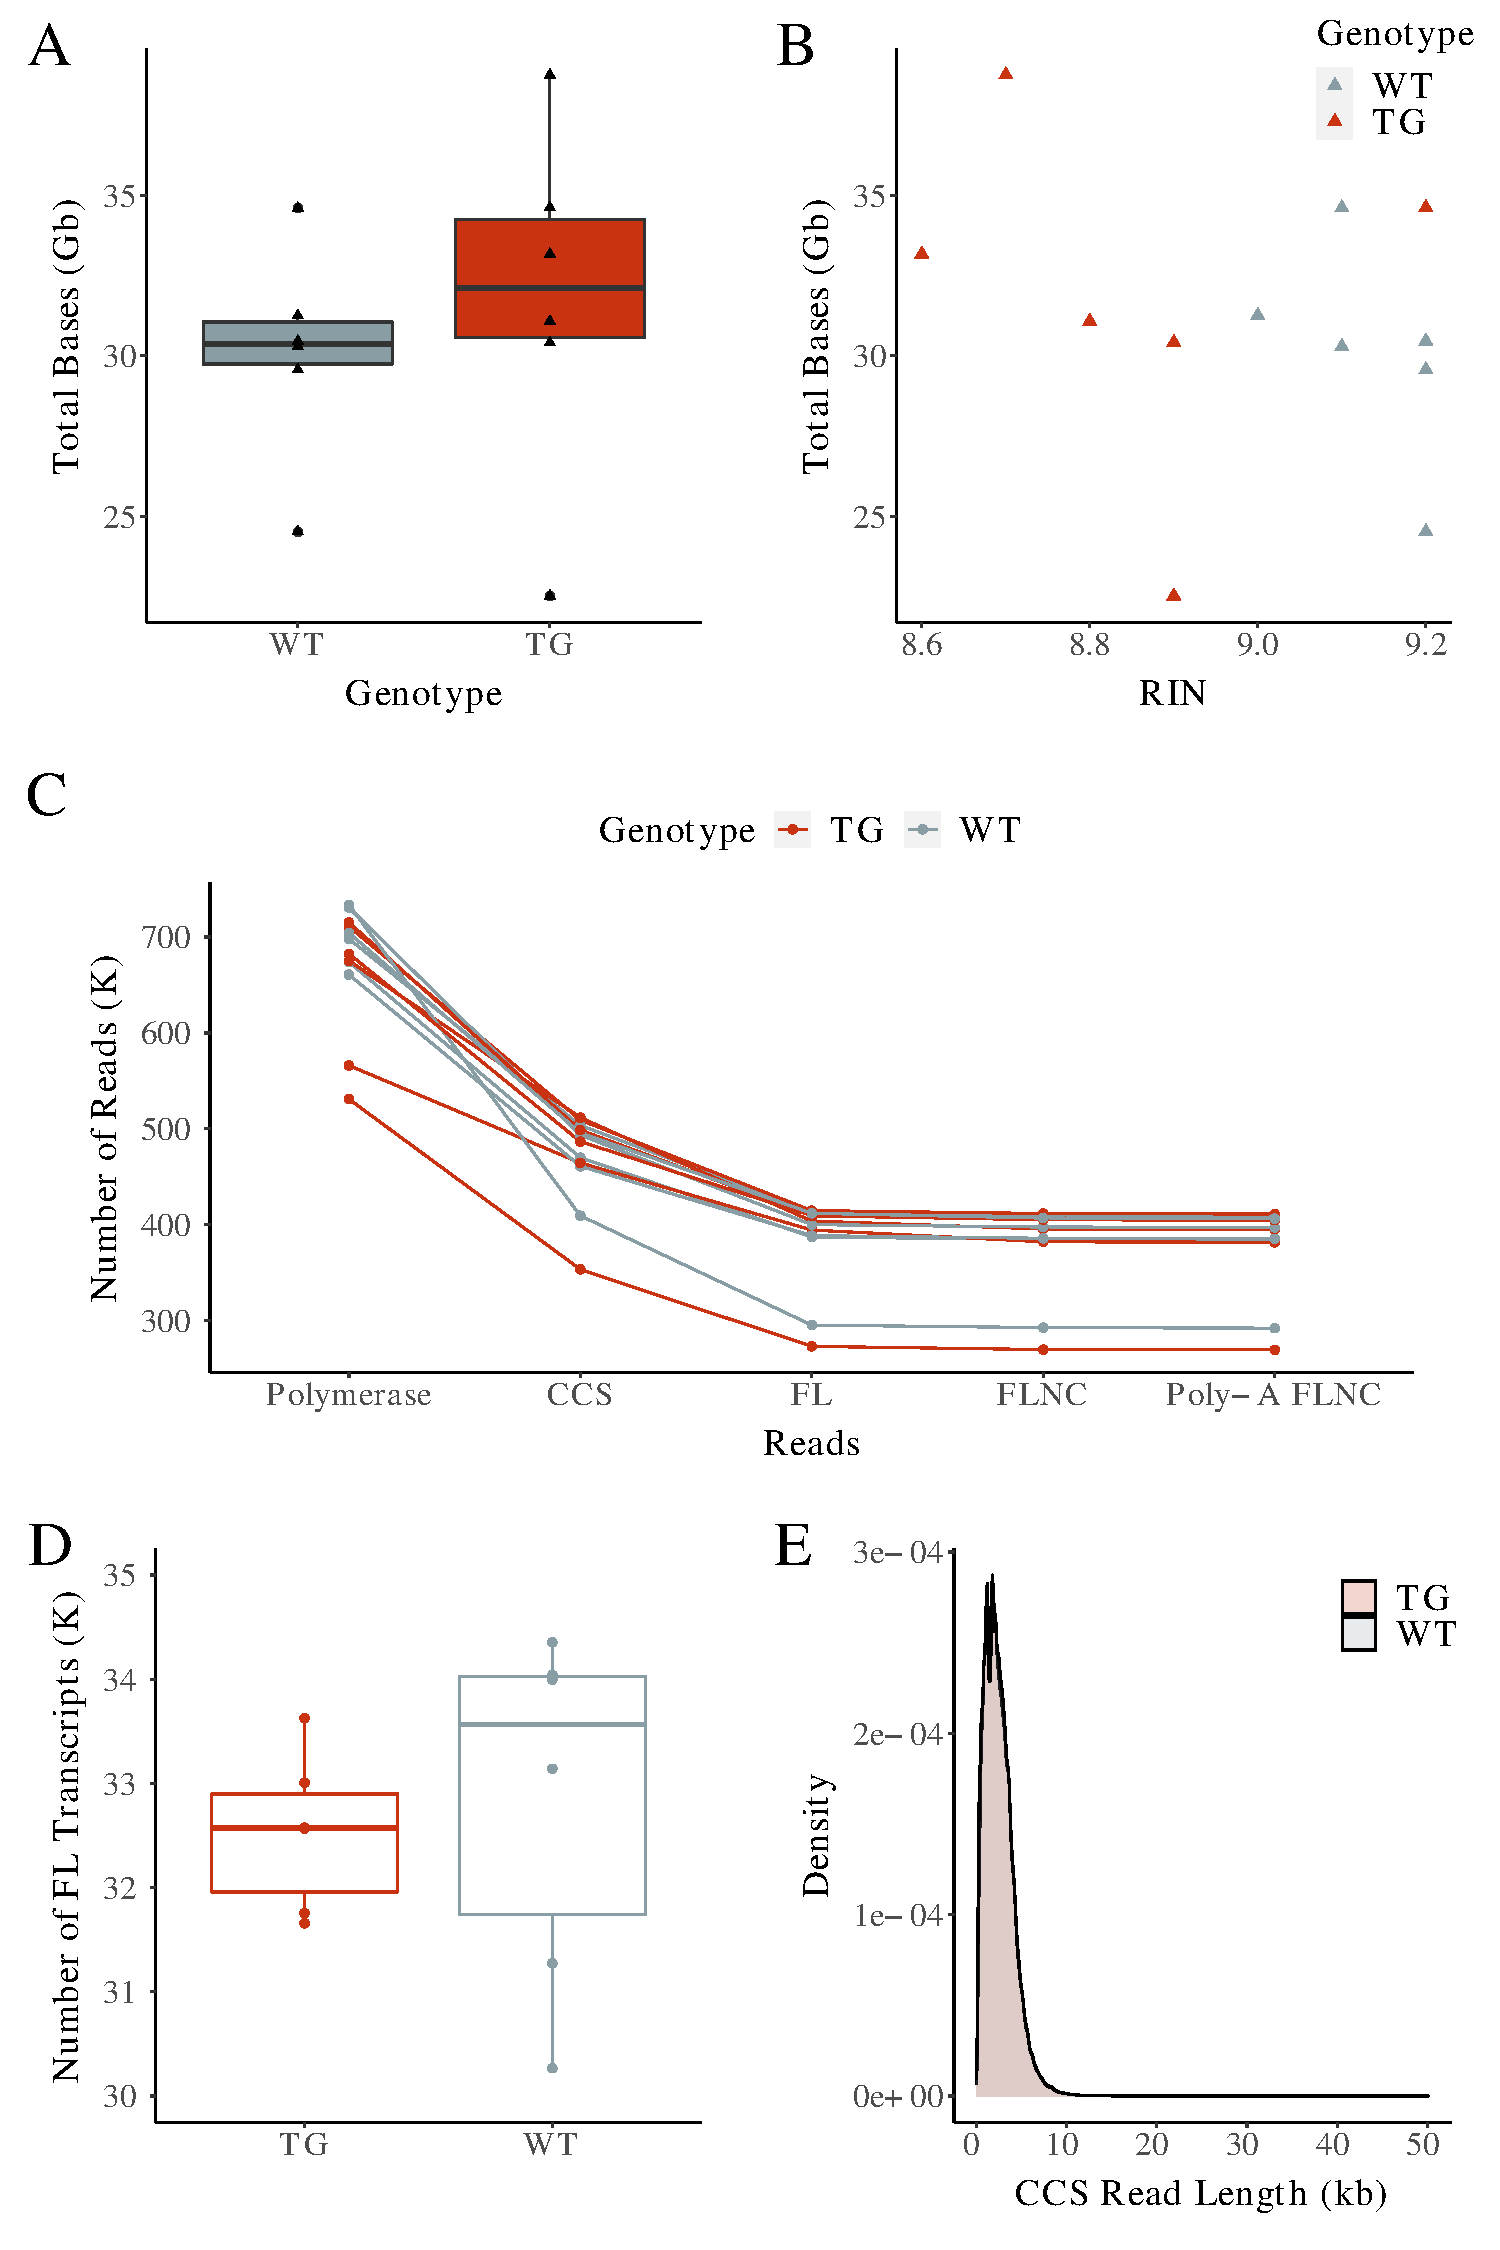
\includegraphics[page=1,trim={0 0 0 0},clip,scale = 0.55]{Figures/rTg4510WholeTranscriptome.pdf}
	\end{center}
	\captionsetup{width=0.95\textwidth}
	\caption[Iso-Seq sequencing metrics from global transcriptome profiling of rTg4510 mice]%
	{\textbf{No significant difference in sequencing metrics, number of transcripts and read length were observed between WT and rTg4501 TG mice}: \textit{Legend continues on the following page.}}
	\label{fig:rTg4510_sequencing_metrics}
\end{figure}
\begin{figure}[p]
	\captionsetup{width=0.95\textwidth}
	\contcaption{Shown is \textbf{(A)} a box plot of the total yield generated from Iso-Seq sequencing of rTg4510 WT (n = 6) and TG mice (n = 6). Full details of all runs are provided in \cref{tab:isoseq_wholerun_result}. \textbf{(B)} A scatter plot of the total yield generated and the RIN attained for each sample (RIN refers to the quality of RNA used for library preparation). \textbf{(C)} The number of reads generated through the Iso-Seq bioinformatics pipeline from initial generation of CCS reads, full-length reads with primer removal to poly(A) FLNC reads with removal of artificial concatemers and trimming of poly(A) tails. Note, the first two samples with lower throughput were sequenced using an older chemistry. \textbf{(D)} A box plot of the total number of full-length transcripts generated for WT and TG mice. \textbf{(E)} Distribution of CCS read length. CCS - Circular consensus sequence, FL - Full-length, FLNC - Full-length non-chimeric, Gb - Gigabases, K - Thousand, kb - Kilobases, TG - rTg4510 transgenic mice, WT - Wild-type mice.}
\end{figure}


\subsection{\textit{MAPT} transgene is only expressed in rTg4510 TG mice}
\label{mapt_transgene_whole}
%Check whether overexpression of human MAPT result in any unwanted, compensatory effects on equivalent mouse genes,as expression levels of mouse APP and MAPT should be slightly reduced, thereby suggesting no evidence that human transgene expression increase expression of directly-related mouse genes.
As expected, human-specific \textit{MAPT} sequences were only detected in reads from TG mice, confirming stable activation of the human \textit{MAPT} transgene (\cref{fig:isoseq_humanmapt}\textbf{A}) and supporting our previous analysis using short-read RNA-Seq data\cite{Castanho2020}. In line with previous results, we also observed a decrease in transgene expression associated with age - a likely reflection of progressive neuronal loss, given that the transgene expression is largely restricted to excitatory neurons under the CAMK2a promoter. Alignment of these human-specific transcripts to the mouse genome were either mapped to the mouse prion protein gene (\textit{Prnp}) with high identity but low alignment length (i.e similar in nucleotide sequence but low overlap, \cref{fig:isoseq_humanmapt}\textbf{B,C}) or to the mouse \textit{Mapt} gene with low identity but high alignment length (i.e not similar in nucleotide sequence but high overlap, \cref{fig:isoseq_humanmapt}\textbf{B,D}). This is reflective of the transgene sequence in rTg4510 mouse model, given it contains exons 2 and 3 of mouse \textit{Prnp}\cite{Ramsden2005} and is homologous to the mouse \textit{Mapt} gene. Applying filter thresholds (85\% alignment identity and 95\% alignment length) for downstream analysis removed these human-specific \textit{MAPT} transcripts (\cref{fig:isoseq_humanmapt}\textbf{B}). 

\begin{figure}[htp]
	\begin{center}
		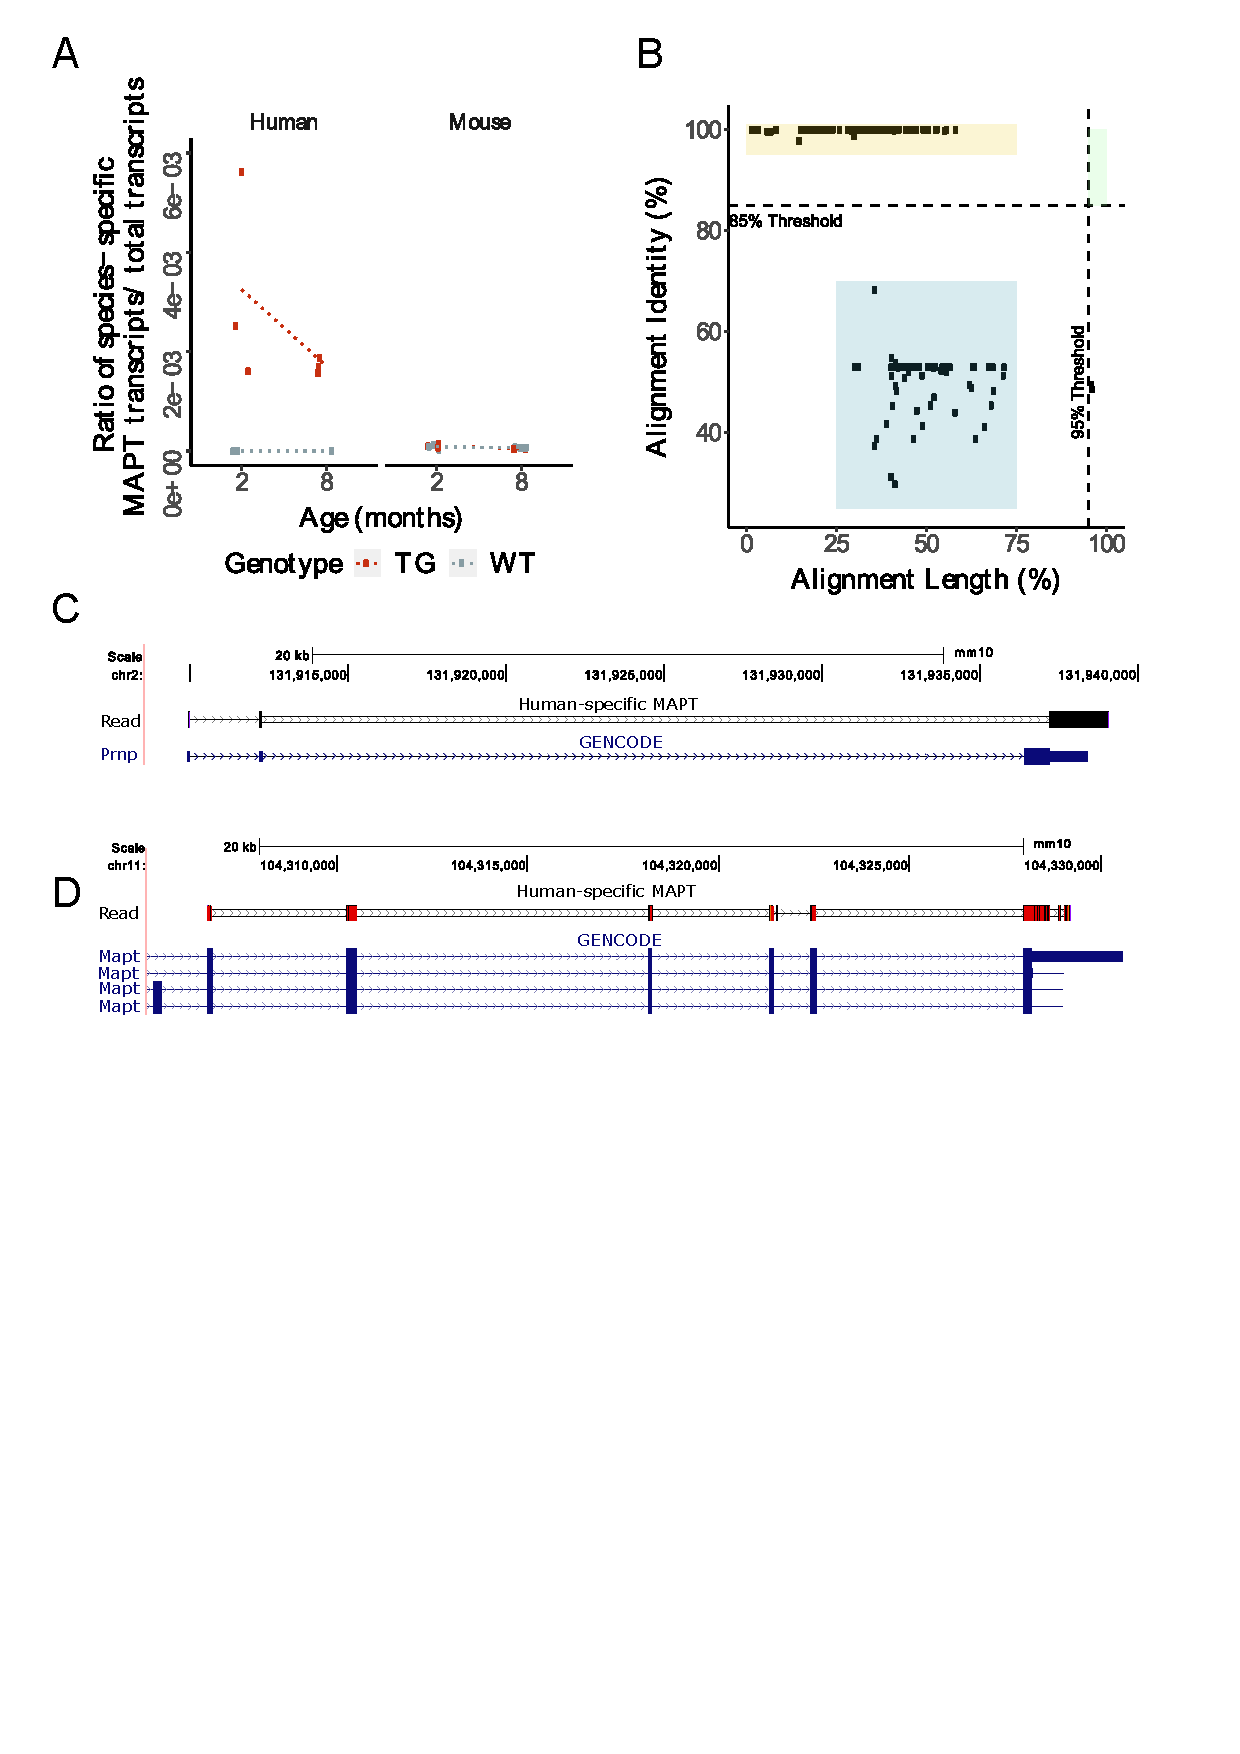
\includegraphics[page=1,trim={0cm 11cm 0cm 0cm},clip,scale = 0.80]{Figures/AltFigures_Diff.pdf}	\end{center}
	\captionsetup{width=0.95\textwidth}
	\caption[Quantifying human-specific \textit{MAPT} sequences in Iso-Seq global dataset]%
	{\textbf{Human-specific \textit{MAPT} sequences were only present in transgenic mice with relatively low homology to mouse \textit{Prnp} and \textit{Mapt} gene.} The presence of human- and mouse-specific \textit{MAPT}/\textit{Mapt} sequences was measured in full-length transcripts generated from Iso-Seq merged dataset. Shown is \textbf{(A)} a scatter plot of the ratio of full-length transcripts that were mapped to human-specific \textit{MAPT} and mouse-specific \textit{Mapt} sequences. Dotted lines represent the mean paths across ages. \textbf{(B)} A scatter plot of the alignment metrics of human-specific \textit{MAPT} transcripts to the mouse genome. Transcripts were either aligned to mouse \textit{Prnp} gene (boxed yellow) with high identity but low length (given that the transgene contains only exon 2 and 3 of mouse \textit{Prnp} gene\cite{Ramsden2005}) or mouse \textit{Mapt} gene (boxed blue) with low alignment identity but relatively high length. Green box refers to the transcripts retained after applying identity and length threshold. \textbf{(C)} UCSC genome browser tracks of human-specific (black) \textit{MAPT} transcripts (transgene) and mouse \textit{Prnp} gene and \textbf{(D)} mouse \textit{Mapt} gene. Blue tracks represent known transcripts from mouse reference genome (mm10). The double horizontal lines indicate unalignable sequences and the red lines indicate bases that differ between the genome and transcript. Tracks were cropped and modified to remove irrelevant genes within the same locus. UTR - Untranslated region.}
	\label{fig:isoseq_humanmapt}
\end{figure}

\clearpage
\subsection{rTg4510 WT and TG mice were characterised with a similar global transcriptomic profile}
\label{ch4: mice_AS_events}
Despite identifying widespread RNA isoform diversity amongst genes expressed in the mouse entorhinal cortex (\cref{ch: whole_transcriptome}), the global transcriptomic profile between rTg4510 WT and TG mice were very similar. No difference was observed in the number of genes (mean n = 13,572 genes) or isoforms (mean n = 53,833 isoforms). Further characterisation of the transcriptome revealed similar profile of isoform diversity across genotype and age (\cref{tab:isoseq_whole_subsqantioutput}), with half of the isoforms annotated as known and FSM (mean n = 30,018 isoforms, 55.8\%, as also shown in \cref{sec:whole_novelIso}) and with a similar distribution of isoform length and exon number (median = 8, range = 1 - 89). Splicing patterns were also very similar across genotype and age with usage of alternative first exons (AF) (mean n = 12,564 AF splicing events, 35\%) (\cref{AS_WholeTranscriptome_diff}) as the most prevalent AS event across all the datasets, in line with previous findings (\cref{sec:whole_novelIso}).

\vspace{2cm}
\begin{table}[!htp]
	\centering
	\captionsetup{width=1\textwidth}
	\caption[Alternative splicing events associated with tau pathology and age]%
	{\textbf{Alternative splicing events associated with tau pathology and age.} Tabulated is the number of splicing events detected for wild-type and rTg4510 transgenic mice aged 2 and 8 months (n = 12 samples, 3 biological replicates per group). Refer to \cref{fig:AS_events} for depiction of the different types of splicing events.}
	\begin{tabular}{@{}ccccc@{}}
		\toprule
		\multirow{2}{*}{Splicing  events} & \multicolumn{2}{c}{Wild-type} & \multicolumn{2}{c}{Transgenic} \\ \cmidrule(l){2-5} 
		& 2 months        & 8 months        & 2 months        & 8 months        \\ \midrule
		A3 & 2164 (6.58\%)   & 2571 (6.61\%)   & 2388 (6.77\%)   & 2388 (6.5\%)    \\
		A5 & 1369 (4.16\%)   & 1589 (4.09\%)   & 1473 (4.18\%)   & 1488 (4.05\%)   \\
		AF & 12048 (36.61\%) & 13073 (33.61\%) & 12514 (35.48\%) & 12622 (34.36\%) \\
		AL & 8140 (24.73\%)  & 9688 (24.91\%)  & 8641 (24.5\%)   & 9287 (25.28\%)  \\
		IR & 3611 (10.97\%)  & 5404 (13.9\%)   & 4293 (12.17\%)  & 4774 (13\%)     \\
		MX & 299 (0.91\%)    & 392 (1.01\%)    & 331 (0.94\%)    & 329 (0.9\%)     \\
		SE & 5278 (16.04\%)  & 6174 (15.88\%)  & 5632 (15.97\%)  & 5846 (15.91\%)  \\ \bottomrule
	\end{tabular}
	\label{AS_WholeTranscriptome_diff}
\end{table}

%stats?
%XX of known transcripts were identified to have intron retention; XX of known transcripts were identified to be fusion genes. XX of know transcripts identified to have non-sense-mediated decay. 

\begin{landscape}
	\begin{table}[]
		\centering
		\captionsetup{width=1\linewidth}
		\caption[Global rTg4510 transcriptome annotations by genotype and age]%
		{\textbf{Transcriptome annotations from global transcriptome profiling of the rTg4510 cortex by genotype and age.} Tabulated is an overview of the Iso-Seq global transcriptome datasets generated from the rTg4510 mouse model, subsected by phenotype and age. Annotations from wild-type mice (n = 6 samples) and rTg4510 transgenic mice (n = 6 samples) were generated from merging Iso-Seq datasets from mouse aged 2 and 8 months of the respective phenotype. Novel genes refer to genes that were not currently present in existing genome annotations (mm10). Isoforms can be further classified as known (FSM, ISM) or novel (NIC, NNC, Genic Genomic, Antisense, Fusion, Intergenic, Genic Intron), as described in \cref{section: sqanti_annotations}. FSM – Full Splice Match, ISM – Incomplete Splice Match, NIC – Novel In Catalogue, NNC – Novel Not in Catalogue.}
		\label{tab:isoseq_whole_subsqantioutput}
		\resizebox{1.6\textwidth}{!}{%
		\begin{tabular}{@{}ccccccc@{}}
		\toprule
		\multicolumn{1}{l}{} &
		\begin{tabular}[c]{@{}c@{}}Wild-type \\ (n = 6)\end{tabular} &
		\begin{tabular}[c]{@{}c@{}}Transgenic \\ (n = 6)\end{tabular} &
		\begin{tabular}[c]{@{}c@{}}Wild-type, 2 months \\ ( n = 3)\end{tabular} &
		\begin{tabular}[c]{@{}c@{}}Wild-type, 8 months \\ ( n = 3)\end{tabular} &
		\begin{tabular}[c]{@{}c@{}}Transgenic, 2 months\\ ( n = 3)\end{tabular} &
		\begin{tabular}[c]{@{}c@{}}Transgenic, 8 months \\ ( n = 3)\end{tabular} \\ \midrule
		Total number of genes             & 14118           & 14213           & 13191           & 13312           & 12985           & 13616           \\
		Known genes                   & 13932 (98.68\%) & 14031 (98.72\%) & 13081 (99.17\%) & 13168 (98.92\%) & 12874 (99.15\%) & 13474 (98.96\%) \\
		Novel genes                       & 186 (1.32\%)    & 182 (1.28\%)    & 110 (0.83\%)    & 144 (1.08\%)    & 111 (0.85\%)    & 142 (1.04\%)    \\
		Total number of isoforms          & 62533           & 63038           & 48516           & 50278           & 45903           & 52730           \\
		FSM                               & 33239 (53.15\%) & 33563 (53.24\%) & 27878 (57.46\%) & 28689 (57.06\%) & 26825 (58.44\%) & 29916 (56.73\%) \\
		ISM                               & 4927 (7.88\%)   & 4864 (7.72\%)   & 3426 (7.06\%)   & 3841 (7.64\%)   & 3279 (7.14\%)   & 3764 (7.14\%)   \\
		NIC                               & 15305 (24.48\%) & 15595 (24.74\%) & 11012 (22.7\%)  & 11407 (22.69\%) & 10214 (22.25\%) & 12369 (23.46\%) \\
		NNC                               & 8518 (13.62\%)  & 8484 (13.46\%)  & 5838 (12.03\%)  & 5953 (11.84\%)  & 5259 (11.46\%)  & 6282 (11.91\%)  \\
		Genic Genomic                     & 63 (0.1\%)      & 61 (0.1\%)      & 44 (0.09\%)     & 44 (0.09\%)     & 32 (0.07\%)     & 47 (0.09\%)     \\
		Antisense                         & 97 (0.16\%)     & 104 (0.16\%)    & 52 (0.11\%)     & 77 (0.15\%)     & 68 (0.15\%)     & 75 (0.14\%)     \\
		Fusion                            & 276 (0.44\%)    & 268 (0.43\%)    & 200 (0.41\%)    & 186 (0.37\%)    & 167 (0.36\%)    & 196 (0.37\%)    \\
		Intergenic                        & 108 (0.17\%)    & 99 (0.16\%)     & 66 (0.14\%)     & 81 (0.16\%)     & 59 (0.13\%)     & 81 (0.15\%)     \\
		Genic Intron                      & 0 (0\%)         & 0 (0\%)         & 0 (0\%)         & 0 (0\%)         & 0 (0\%)         & 0 (0\%)         \\
		Isoform length (bp) &
		\begin{tabular}[c]{@{}c@{}}Median: 2691, \\ Range: 82-15016\end{tabular} &
		\begin{tabular}[c]{@{}c@{}}Median: 2698, \\ Range: 82-15913\end{tabular} &
		\begin{tabular}[c]{@{}c@{}}Median: 2740, \\ Range: 88-15016\end{tabular} &
		\begin{tabular}[c]{@{}c@{}}Median: 2614, \\ Range: 82-14850\end{tabular} &
		\begin{tabular}[c]{@{}c@{}}Median: 2548, \\ Range: 88-14302\end{tabular} &
		\begin{tabular}[c]{@{}c@{}}Median: 2754, \\ Range: 82-15913\end{tabular} \\
		Number of exons &
		\begin{tabular}[c]{@{}c@{}}Median: 8, \\ Range: 1-89\end{tabular} &
		\begin{tabular}[c]{@{}c@{}}Median: 8, \\ Range: 1-89\end{tabular} &
		\begin{tabular}[c]{@{}c@{}}Median: 9, \\ Range: 1-89\end{tabular} &
		\begin{tabular}[c]{@{}c@{}}Median: 8, \\ Range: 1-89\end{tabular} &
		\begin{tabular}[c]{@{}c@{}}Median: 8, \\ Range: 1-77\end{tabular} &
		\begin{tabular}[c]{@{}c@{}}Median: 9, \\ Range: 1-89\end{tabular} \\
		Number of isoforms within 50bp CAGE & 52096 (83.31\%) & 52633 (83.49\%) & 40589 (83.66\%) & 42378 (84.29\%) & 38227 (83.28\%) & 44729 (84.83\%) \\ \bottomrule
	\end{tabular}%
		}
		\end{table}
\end{landscape}

 
\subsection{Iso-Seq confirms widespread gene expression differences associated with tau pathology in rTg4510 mice detected using short-read RNA-Seq}
\label{ch5: diffgeneexp}
%\boldheader{Usage of Iso-Seq reads alone detected robust changes in gene expression}
Although long-read sequencing is often assumed to be less quantitative than traditional short-read RNA-Seq approaches, we previously demonstrated the power of Iso-Seq to accurately quantify the abundance of highly-expressed transcripts (as described in \cref{sec: whole_isoseqvsrnaseq}). Subsequently, we sought to evaluate the utility of full-length Iso-Seq read counts as a proxy of abundance to identify differences in gene expression associated with progressive tau pathology. Of note, a recent RNA-Seq study by our group identified extensive gene expression differences in the same mouse model using short-read RNA-Seq data mapped to the mouse reference genome annotation\cite{Castanho2020}.

Using Iso-Seq read counts as a proxy of abundance (as detailed in \cref{sec: gene_isoform_quant_explained}), we identified 483 genes differentially expressed at a stringent FDR < 0.05. Using \textit{MasigPro} to differentiate genotype and age effects (as illustrated in \cref{fig:dea_model}), we identified evidence for differential gene expression associated with the rTg4510 genotype (\cref{fig:dea_model_genexp}\textbf{A,B}) and age (\cref{fig:dea_model_genexp}\textbf{B,C}), and interactions between genotype and age (\cref{fig:dea_model_genexp}\textbf{D,E,F,G}). Classifying differentially expressed genes by effects, we identified 18 (3.73\%) differentially expressed genes that were associated with genotype effect, and 356 (73.7\%) genes whose expression significantly altered with tau pathology progression in rTg4510 mice (i.e interaction effect) (\cref{fig:dea_model_num}). Among these, there was a significant (Exact bionomial test: n = 356 genes, \textit{P} = 1.91 x 10\textsuperscript{-44}) enrichment of up-regulated genes (n = 304 genes (85.3\%) with increased expression in TG compared to WT; n = 52 (14.6\%) genes with decreased expression in TG). Using \textit{EnrichR}, the differentially expressed genes were found to be highly enriched in the lysosome (GO Cellular Component: adjusted \textit{P} = 4.19 x 10\textsuperscript{-4}, odds ratio = 3.06) and in particular, the TGF-$\beta$  signalling pathway (WikiPathway 2021 Human: adjusted \textit{P} = 2.92 x 10\textsuperscript{-2}, odds ratio = 17.16). Further in line with previous findings, a third of the differentially expressed genes were enriched in pathways involved in immune system activation (n = 140 genes, 34.4\% of genes identified in the “turquoise” co-expression module\cite{Castanho2020}, \cref{fig:dea_model_num}\textbf{B}). 

Our previous RNA-Seq study\cite{Castanho2020} was more powered with a bigger sample size (RNA-Seq: n = 30 WT, n = 29 TG; Iso-Seq: n = 6 WT, n = 6 TG) and a deeper sequencing coverage (RNA-Seq: mean number of reads = 18.8M; Iso-Seq: mean number of CCS reads = 5.7M reads) and unsurprisingly identified a larger number of gene expression differences (n = 1,916 differentially expressed genes). However, 116 (6.05\%) of these genes were also detected as differentially expressed using normalised Iso-Seq read counts as a proxy of expression, illustrating the utility of long-read sequencing for gene quantification and gene-level analyses. Recapitulating findings from our previous RNA-Seq study, we also identified \textit{Gfap} and \textit{C4b} as top-ranked differentially expressed genes associated with progressive tau pathology. Up-regulation of \textit{Gfap} (\cref{fig:whole_dea}\textbf{A,B}) - which encodes for the glial fibrillary acidic protein, a cytoskeletal protein that acts as a marker for astrocyte activation - and \textit{C4b} (\cref{fig:whole_dea}\textbf{C,D}) - a member of the complement immune system - have also been previously observed in human AD post-mortem brain tissue and other AD mouse models\cite{Muramori1998,Ishiki2016, Chatterjee2021}. Other top-ranked differentially expressed genes, whose expression differences were also recapitulated using Iso-Seq full-length read counts (\cref{tab:dea_wholemouse}), included: i) \textit{Slc14a1}\cite{Castillo2017} encoding the urea transporter 1, ii) \textit{Tgfbr1} encoding the TGF-\textbeta receptor protein (\cref{fig:whole_dea}\textbf{E,F}), and iii) \textit{Unc93b1}\cite{Wirz2013}, a transmembrane protein required for the toll pathway.

\begin{figure}[h]
	\centering
	\includegraphics[page=5,scale = 0.55]{Figures/WholeDifferentialAnalysis.pdf}
	\captionsetup{width=0.95\textwidth}
	\caption[Examples of differential expression associated with genotype, age \& interaction effects]%
	{\textbf{Differentially expressed genes exhibiting genotype, age and interaction effects.} Shown are examples of differentially expressed genes classified under the different models using the Iso-Seq global transcriptome profiling (n = 6 WT, n = 6 TG, across age 2 and 8 months) with Iso-Seq full-length read counts for quantification: \textbf{(A)} \textit{Tigd2} with a genotype effect, \textbf{(B)} \textit{Mobp} with a genotype and age effect, \textbf{(C)} \textit{Cik1} with an age effect, and \textbf{(D)} \textit{Cd34}, \textbf{(E)} \textit{Unc93b1}, \textbf{(F)} \textit{Csf1r} and \textbf{(G)} \textit{Tgfbr2} with an interaction effect. Dashed lines represent mean paths across age groups. Wild-type and rTg4510 transgenic mice are denoted by red and grey, respectively. The models are defined using \textbf{Equation 5.1} and depicted in \cref{fig:dea_model}.}   
	\label{fig:dea_model_genexp}
\end{figure}
 
\begin{figure}[h]
	\centering
	\includegraphics[page=4,trim={0 19cm 0 0},clip,scale = 0.55]{Figures/WholeDifferentialAnalysis.pdf}
	\captionsetup{width=0.95\textwidth}
	\caption[Differentially expressed genes classified by conditions]%
	{\textbf{Differentially expressed genes were identified across all the different conditions with a number of differentially expressed genes exhibiting an interaction effect of rTg4510 genotype and age.} \textbf{(A)} A bar chart of the number of differentially expressed genes (n = 483), determined from Iso-Seq FL read count as a proxy of expression and classified by rTg4510 genotype, age, and interaction effect (n = 6 WT, n = 6 TG, across 2 and 8 months). \textbf{(B)} A pie chart of the number and proportion of differentially expressed genes with genotype and interaction effect (n = 407 genes) identified in discrete co-expression network modules taken from our previous RNA-Seq study\cite{Castanho2020}; all three modules were significantly associated with progressive tau pathology: the “Red” module was down-regulated in TG mice and enriched for synaptic transmission, the “Turquoise” module was up-regulated in TG mice and enriched for immune system activation, and the “Yellow” module was down-regulated in TG mice and enriched for mitochondrial and synpatic processes. These modules refer to clusters of highly-correlated genes, which were determined using weighted gene correlation network analysis (WGCNA)\nomenclature{WGCNA}{Weighted gene correlation network analysis}\cite{Langfelder2008} and functionally-annotated using gene ontology (GO) analyses\cite{Young2010}.}    
	\label{fig:dea_model_num}
\end{figure}


\begin{figure}[h]
	\begin{center}
		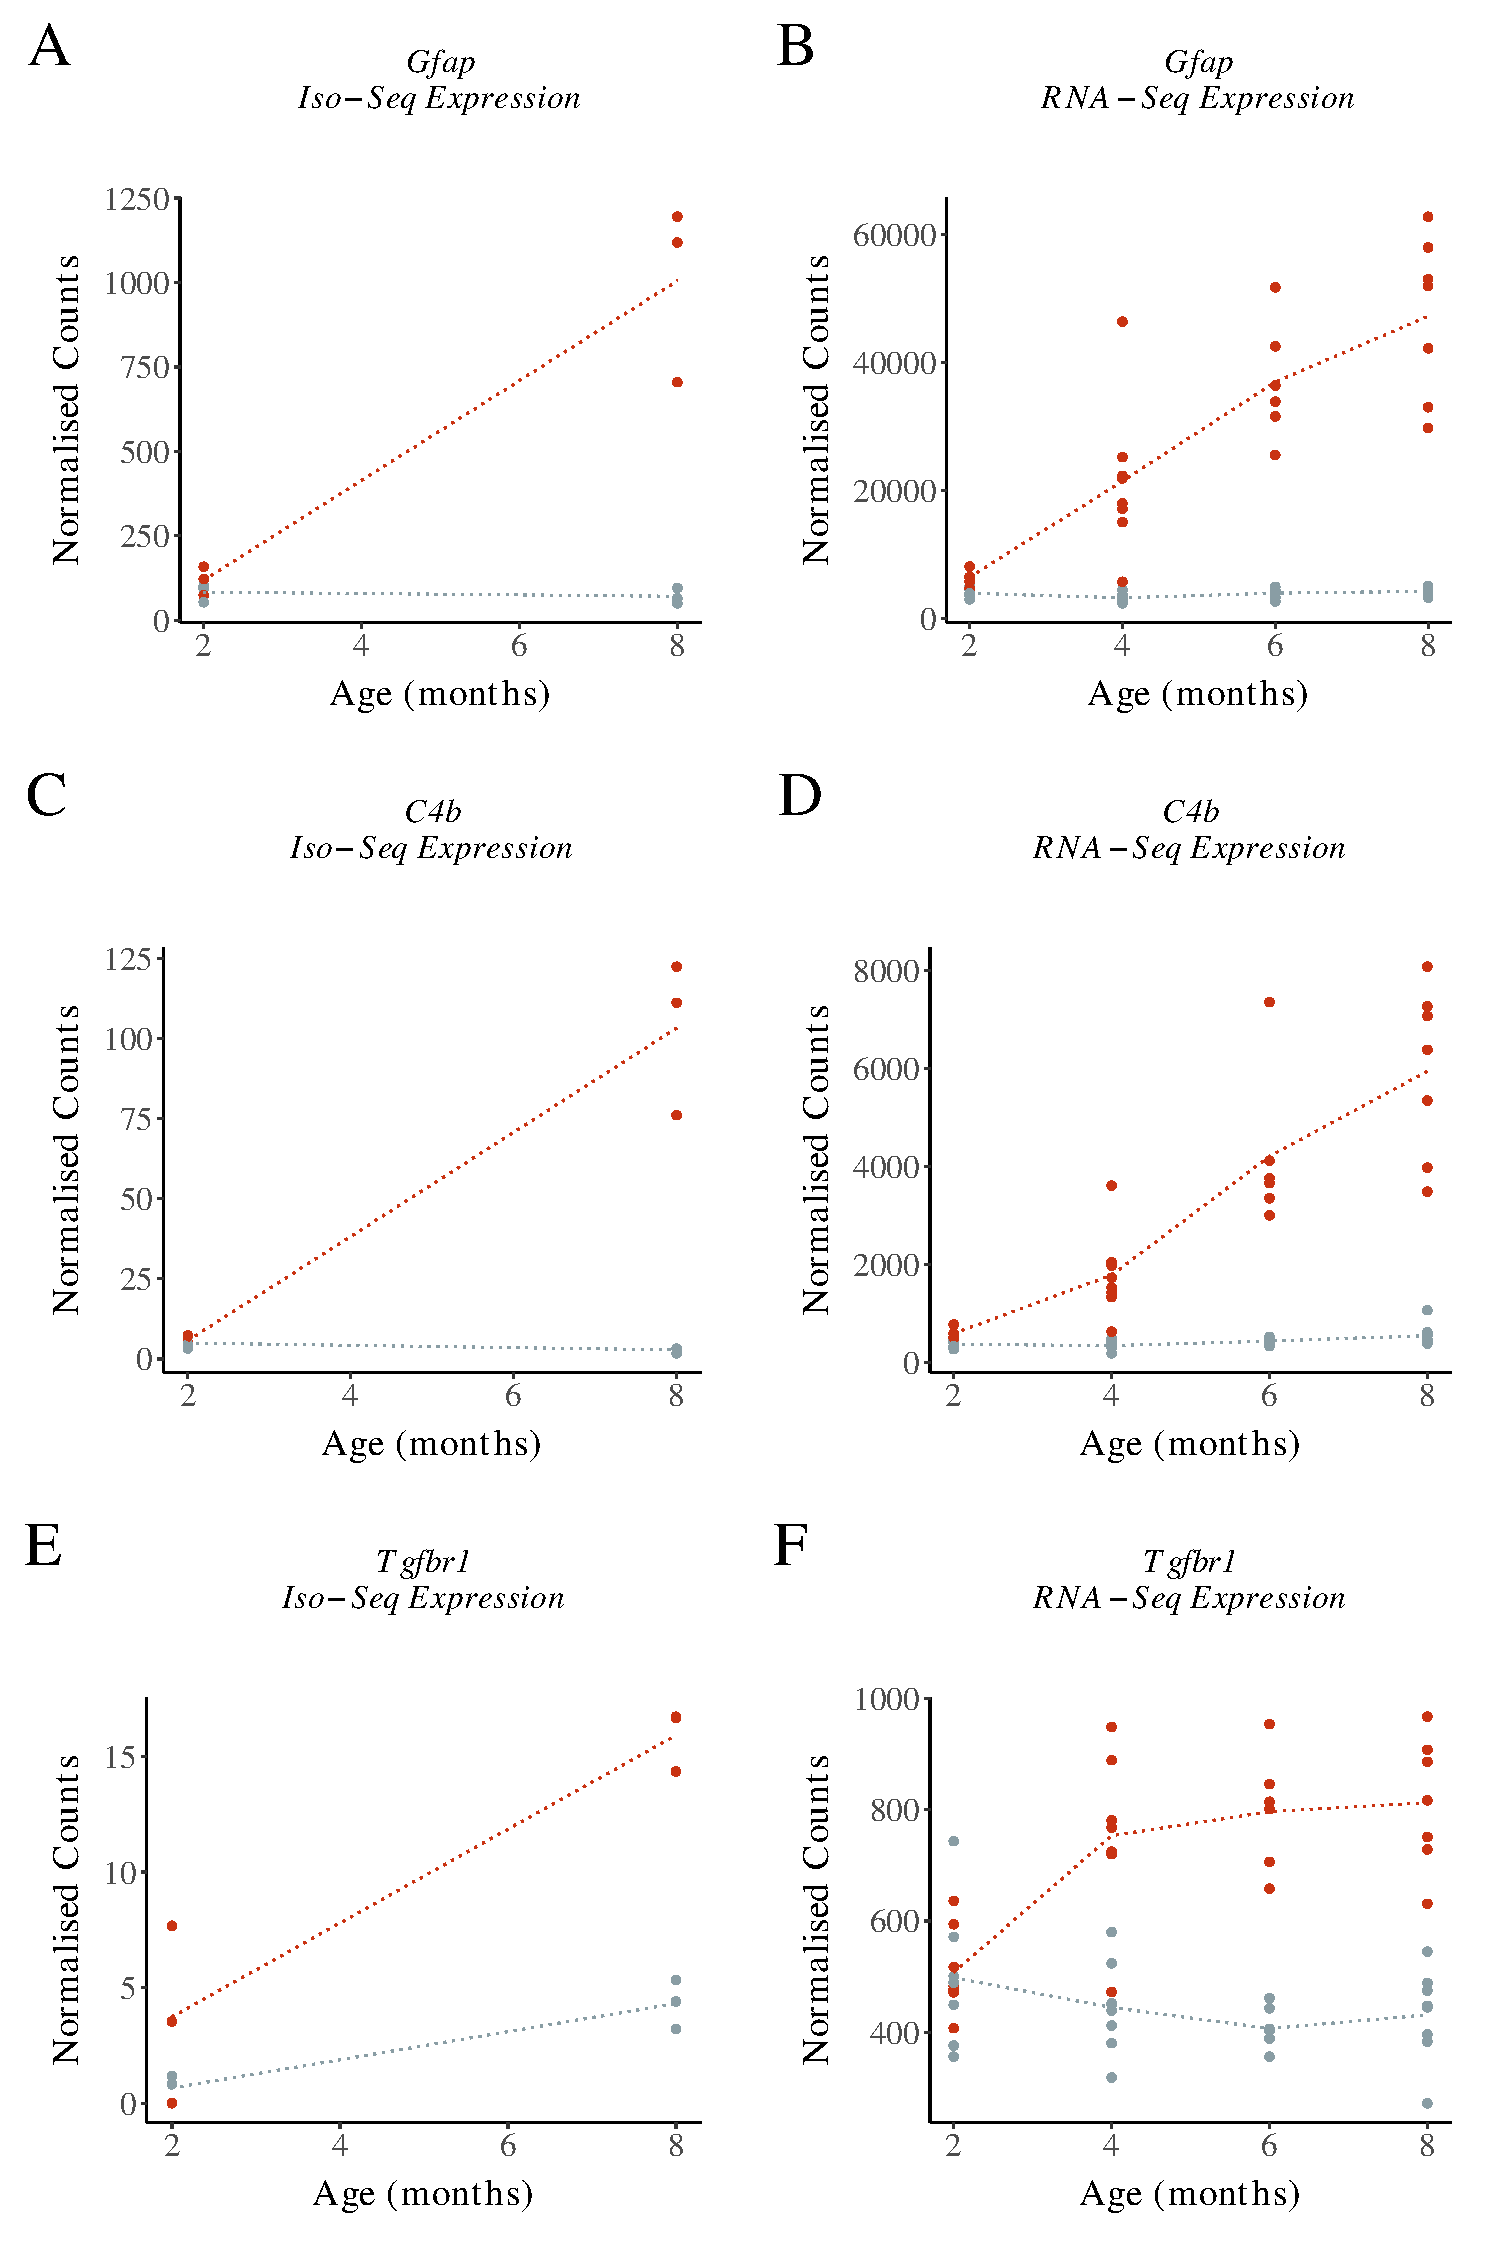
\includegraphics[page=1,scale = 0.55]{Figures/WholeDifferentialAnalysis.pdf}
	\end{center}
	\captionsetup{width=0.95\textwidth}
	\caption[Top-ranked differentially expressed genes associated with rTg4510 genotype]%
	{\textbf{\textit{Gfap} and \textit{C4b} were the top-ranked differentially expressed genes associated with progressive tau pathology in the rTg4510 mice.} Shown are scatter plots of the gene expression for \textbf{(A, B)} \textit{Gfap}, \textbf{(C, D)} \textit{C4b} and \textbf{(E, F)} \textit{Tgfbr1} using either Iso-Seq full-length read count or RNA-Seq reads for transcript quantification. Dashed lines represent mean paths across age groups. Wild-type and rTg4510 transgenic mice are denoted by red and grey, respectively.}   
	\label{fig:whole_dea}
\end{figure}

\vspace{2cm}
%log2fc calculated by mean expression at 8 case/mean expression at 8 control
\begin{table}[!htp]
	\centering
	\captionsetup{width=0.95\textwidth}
	\setlength\tabcolsep{3.5pt} %reduced margin size in table
	\caption[Top-ranked differentially expressed genes associated with rTg4510 genotype]%
	{\textbf{Top-ranked differentially expressed genes associated with rTg4510 genotype.} Tabulated is a summary of the top-ranked genes identified as differentially expressed in rTg4510 mice using \textit{maSigPro} with Iso-Seq-derived transcriptome for annotation and Iso-Seq FL read count for quantification. Gene expression is determined from the sum of normalised expression of associated transcripts.}
	\begin{threeparttable}
	\begin{tabularx}{0.95\textwidth}{cccccccc}
	\toprule
	\multirow{3}{*}{Gene} &
	\multirow{3}{*}{FDR\tnote{a}} &
	\multirow{3}{*}{R\textsuperscript{2}\tnote{,b}} &
	\multirow{3}{*}{\begin{tabular}[c]{@{}c@{}}log\textsubscript{2} FC\textsubscript{genotype}\tnote{c}\end{tabular}} &
	\multicolumn{4}{c}{Mean gene expression} \\ \cmidrule(l){5-8} 
	&          &       &      & \multicolumn{2}{c}{Wild-type} & \multicolumn{2}{c}{Transgenic} \\ \cmidrule(l){5-8} 
	&          &       &      & 2 months      & 8 months      & 2 months       & 8 months      \\ \midrule
	\textit{C4b}    & 1.6 x 10\textsuperscript{-41}  & 0.945 & 4.38 & 4.94          & 2.73          & 4.97           & 103           \\
	\textit{Gfap}     & 6.04 x 10\textsuperscript{-36} & 0.933 & 3.12  & 82.8          & 70.5          & 118            & 1030           \\
	\textit{Tgfbr1}  & 7.9 x 10\textsuperscript{-24}  & 0.892 & 2.95 & 0.663         & 3.38          & 2.03           & 15.7          \\
	\textit{Slc14a1} & 4.31 x 10\textsuperscript{-22} & 0.899 & 2.95 & 9.55          & 14.7          & 6.16           & 47.7            \\
	\textit{Pros1} & 1.05 x 10\textsuperscript{-17} & 0.894 & 2.08 & 8.17          & 9.32         & 6.26           & 26.4          \\
	\textit{Unc93b1} & 1.46 x 10\textsuperscript{-16} & 0.863 & 1.61  & 3.59          & 5.04          & 6.47          & 19.8          \\ \bottomrule
	\end{tabularx}
	\begin{tablenotes}
	\footnotesize
	\item[a] False discovery rate
	\item[b] R\textsuperscript{2} is a statistical measure that represents the amount
	of variance explained by the model
	\item[c] log\textsubscript{2} fold change of TG aged 8 months vs WT aged 8 months
	\end{tablenotes}
	\end{threeparttable}
	\label{tab:dea_wholemouse}
\end{table}

\clearpage
\subsection{rTg4510 mice characterised by expression differences in novel, antisense genes}
Highlighting the power of long-reads to comprehensively annotate the transcriptome, we previously detected novel genes in our Iso-Seq dataset that were not present in existing genome annotations (\cref{sec:whole_novelgenes}). These genes were often lowly-expressed and typically antisense to known genes with overlap at the UTR or gene body (as illustrated in \cref{fig:isoseq_whole_novelfusion}). Given the improved transcript annotation afforded by our Iso-Seq data, we next sought to test for expression differences in these novel genes associated with rTg4510 genotype. This was achieved by quantifying levels of expression by mapping RNA-Seq reads to our improved Iso-Seq-derived transcriptome annotation. 

We identified three of these novel genes with evidence for differential expression associated with rTg4510 genotype. The most significant differentially expressed novel gene was located on chromosome 10 (PB.1799.1, \cref{fig:whole_novelgene_difftracks}\textbf{A}) and was characterised by progressive down-regulation in TG mice (\cref{fig:whole_novelgene_diffexp}\textbf{A}). The other two differentially expressed novel genes were found antisense to known genes: \textit{Fgfr1op} (PB.6616.1, \cref{fig:whole_novelgene_difftracks}\textbf{B}) within the gene-body and \textit{Htra1} at the 5' UTR (PB.15002.1, \cref{fig:whole_novelgene_difftracks}\textbf{C}). Both genes were up-regulated with progressive tau pathology in TG mice (\cref{fig:whole_novelgene_diffexp}\textbf{B,D}). Notably, while \textit{Fgfr1op} was not identified as differentially expressed (\cref{fig:whole_novelgene_diffexp}\textbf{C}), \textit{Htra1} was also found to have a higher expression in rTg4510 TG compared to WT mice (\cref{fig:whole_novelgene_diffexp}\textbf{E}).     
%Htra1-AS shared exonic regions with Htra1 so misalignment of RNA-Seq reads

\begin{landscape}
	\begin{figure}[!htp]
		\centering
		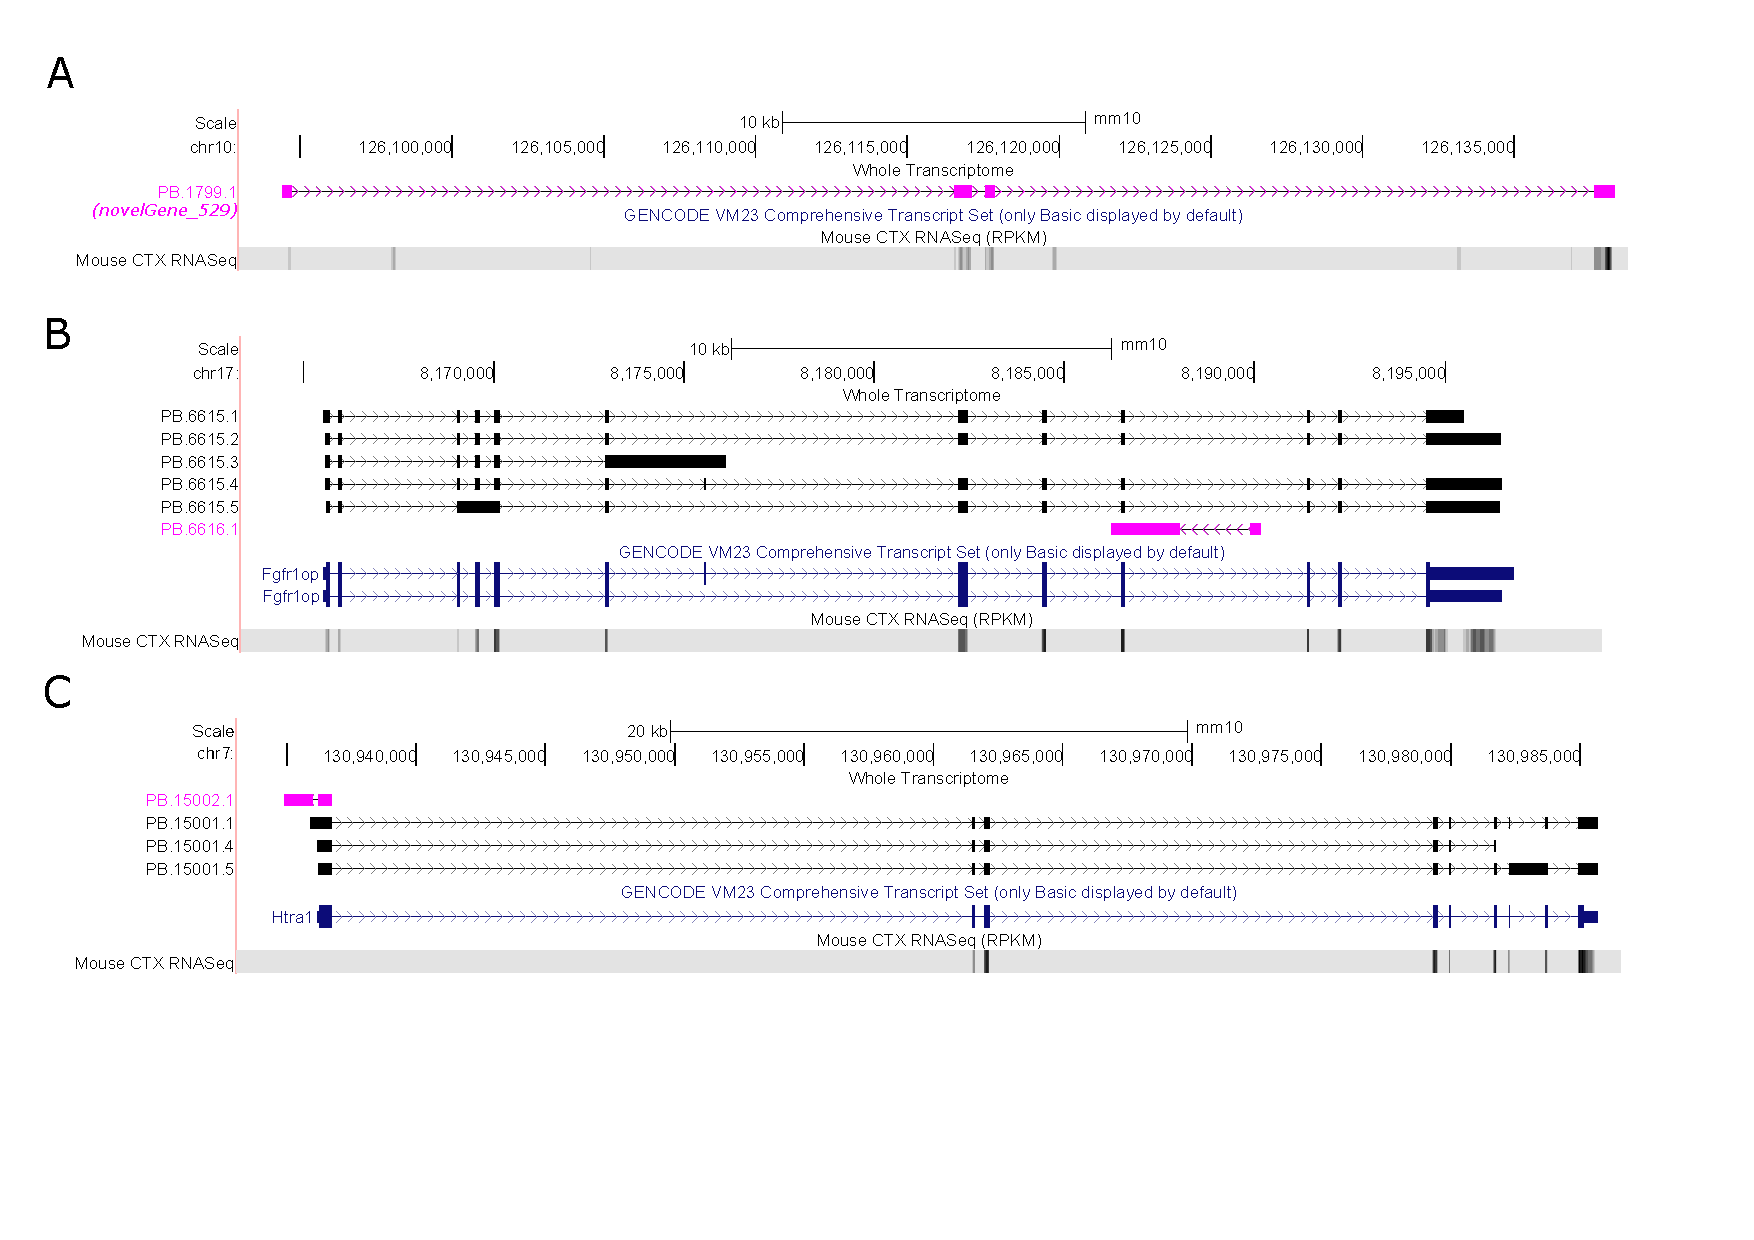
\includegraphics[page=1,trim={0 3.5cm 0 1cm}, scale = 0.80]{Figures/TracksFigures_Diff.pdf}
		\captionsetup{width=1.4\textwidth}
		\caption[Visualisation of differentially expressed novel genes]%
		{\textbf{Visualisation of novel genes that were differentially expressed.} Shown are UCSC genome browser tracks of three differentially expressed novel genes (coloured pink): \textbf{(A)} novel gene on chromosome 10, \textbf{(B)} novel gene antisense to \textit{Fgfr1op}, and \textbf{(C)} novel gene antisense to \textit{Htra1}. Shown are also mouse reference genome annotations (mm10) and RNA-Seq data from matched samples.}   
		\label{fig:whole_novelgene_difftracks}
	\end{figure}
\end{landscape}

\begin{figure}[!htp]
	\begin{center}
		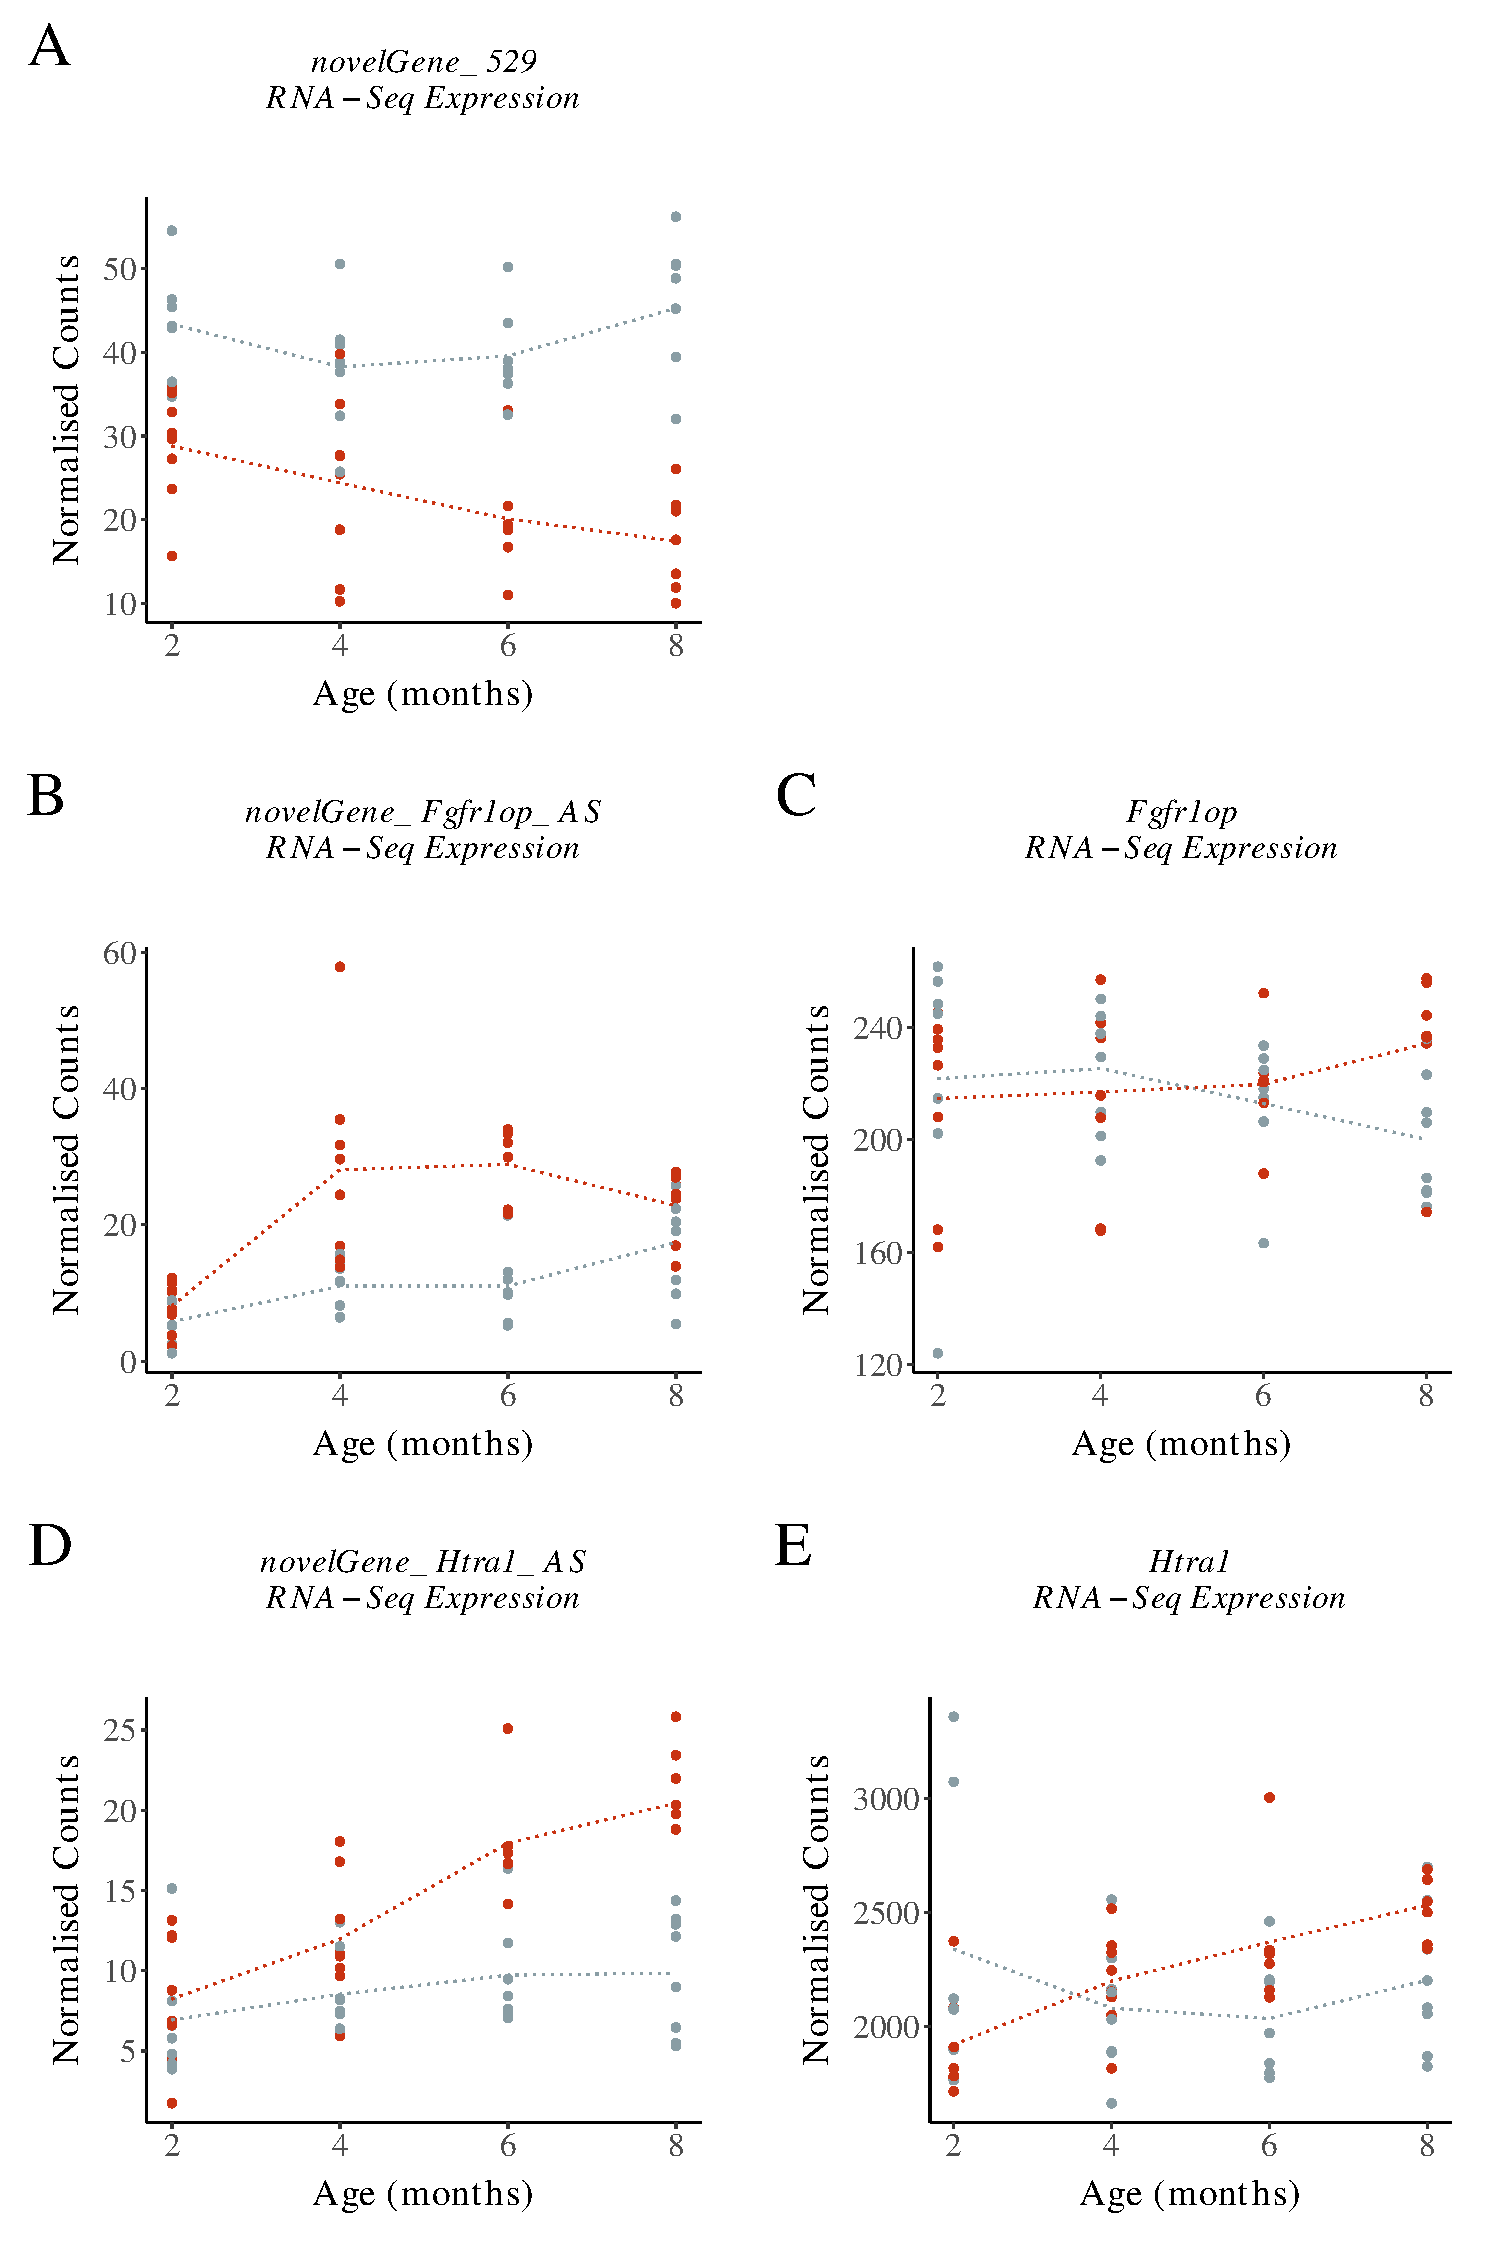
\includegraphics[page=1,scale = 0.55]{Figures/NovelGeneExp.pdf}
	\end{center}
	\captionsetup{width=0.95\textwidth}
	\caption[Differentially expressed novel genes associated with progressive tau pathology]%
	{\textbf{Three novel genes were found differentially expressed in rTg4510 mice.} Shown are scatter plots of three differentially expressed novel genes, located \textbf{(A)} in chromosome 10 (PB.1799.1, \cref{fig:whole_novelgene_difftracks}\textbf{A}), \textbf{(B)} antisense to \textit{Fgfr1op} (PB.6616.1, \cref{fig:whole_novelgene_difftracks}\textbf{B}) and \textbf{(D)} to \textit{Htra1} (PB.15002.1, \cref{fig:whole_novelgene_difftracks}\textbf{C}). Gene expression for the two known genes, \textbf{(C)} \textit{Fgfr1op} and \textbf{(E)} \textit{Htra1}, are also shown. Gene expression was determined from mapping RNA-Seq reads to Iso-Seq-derived annotations.}   
	\label{fig:whole_novelgene_diffexp}
\end{figure}


\clearpage
\subsection{Gene expression differences in rTg4510 mice were primarily driven by the differential expression of dominant isoform}
One of the added advantages of long-read sequencing is the improved confidence to reliably identify isoforms with significant expression differences across experimental conditions. Given that we were able to reliably detect tau-associated differentially expressed genes in rTg4510 TG mice using normalised full-length long-read read counts (described in \cref{ch5: diffgeneexp}), we subsequently sought to identify differentially expressed \textit{transcripts} using the same approach. 

By performing differential transcript expression analysis using \textit{tappAS} with Iso-Seq reads for annotation and quantification, we identified 886 differentially expressed transcripts. Among these, 673 (75.9\%) transcripts were associated with progressive tau pathology (interaction effect), 43 (4.85\%) transcripts with tau pathology (genotype effect) and 170 (19.2\%) transcripts with age. Similar to the gene-level analyses (\cref{ch5: diffgeneexp}), there was a significant (Exact bionomial test: n = 673 transcripts, \textit{P} = 1.72 x 10\textsuperscript{-42}) enrichment of up-regulated transcripts (n = 510 transcripts (75.8\%) increased in TG compared to WT mice). Using \textit{EnrichR}, the differentially expressed transcripts were found to be highly enriched in the lysosome (GO Cellular Component: adjusted \textit{P} = 1.65 x 10\textsuperscript{-4}, odds ratio = 3.25), and in several molecular functions including protein kinase binding (adjusted \textit{P} = 0.048, odds ratio = 2.02) and ATPase binding (adjusted \textit{P} = 0.048, odds ratio = 4.23).  

Two of the most significant differentially expressed transcripts associated with the progression of tau pathology (\cref{tab:DEI_trans}) were annotated to \textit{Gfap} (\cref{fig:DEI_gfap}) and \textit{C4b} (\cref{fig:DEI_c4b}), the top two most differentially expressed genes (\cref{tab:dea_wholemouse}). Both genes were characterised by a dominant known isoform in rTg4510 mice: Gfap-201 (ENSMUST00000077902.5, PB.2972.16) (\cref{fig:DEI_gfap}\textbf{A,B}) and C4b-201 (ENSMUST00000069507.8, PB.7004.8) (\cref{fig:DEI_c4b}\textbf{A,B}). The expression of these two known isoforms were significantly higher than that of the novel isoforms, and were strongly up-regulated with progressive tau pathology (\cref{fig:DEI_gfap}\textbf{D}, \cref{fig:DEI_c4b}\textbf{D}). This suggests that increased \textit{Gfap} (\cref{fig:whole_dea}\textbf{A}) and \textit{C4b} gene expression in aged rTg4510 TG mice were primarily driven by the up-regulation of their respective dominant isoform. This corroborates with previous studies that reported a differential increase in the human-equivalent Gfap-201 transcript in AD temporal cortex\cite{Roelofs2005}, and qPCR studies in AD mouse models that similarly showed up-regulation of \textit{Gfap}-associated isoforms\cite{Kamphuis2012}. Of note, all the other minor novel isoforms were more abundant in the aged rTg4510 transgenic mice (\cref{fig:DEI_gfap}\textbf{C}, \cref{fig:DEI_c4b}\textbf{C}).

These findings were validated with usage of normalised RNA-Seq read counts, after alignment to the improved Iso-Seq-derived transcriptome annotation, as a proxy of expression; both Gfap-201 (\cref{fig:DEI_gfap}\textbf{E}) and C4b-201 (\cref{fig:DEI_c4b}\textbf{E}) were found to be dramatically up-regulated with progressive tau pathology. However, some of the minor novel isoforms annotated to \textit{Gfap} were also found to change with rTg4510 genotype with a more pronounced up-regulation than Gfap-201 (PB.2972.8, PB.2972.17, \cref{fig:DEI_gfap}\textbf{E}). Visualisation of these novel differentially expressed isoforms revealed that they were generally very similar (\cref{fig:DEI_gfap}\textbf{A}), with an almost identical internal exonic structure; for example, PB.2972.8 and Gfap-201 only differed by the presence of exon 3, whereas PB.2972.17 contained an alternative splice site at exon 8. The sensitivity of RNA-Seq reads to differentiate these almost-identical isoforms is therefore questionable, given that there are only a few loci that can be used for unambiguous assignment of short RNA-Seq reads.  

\begin{figure}[!htp]
	\centering
	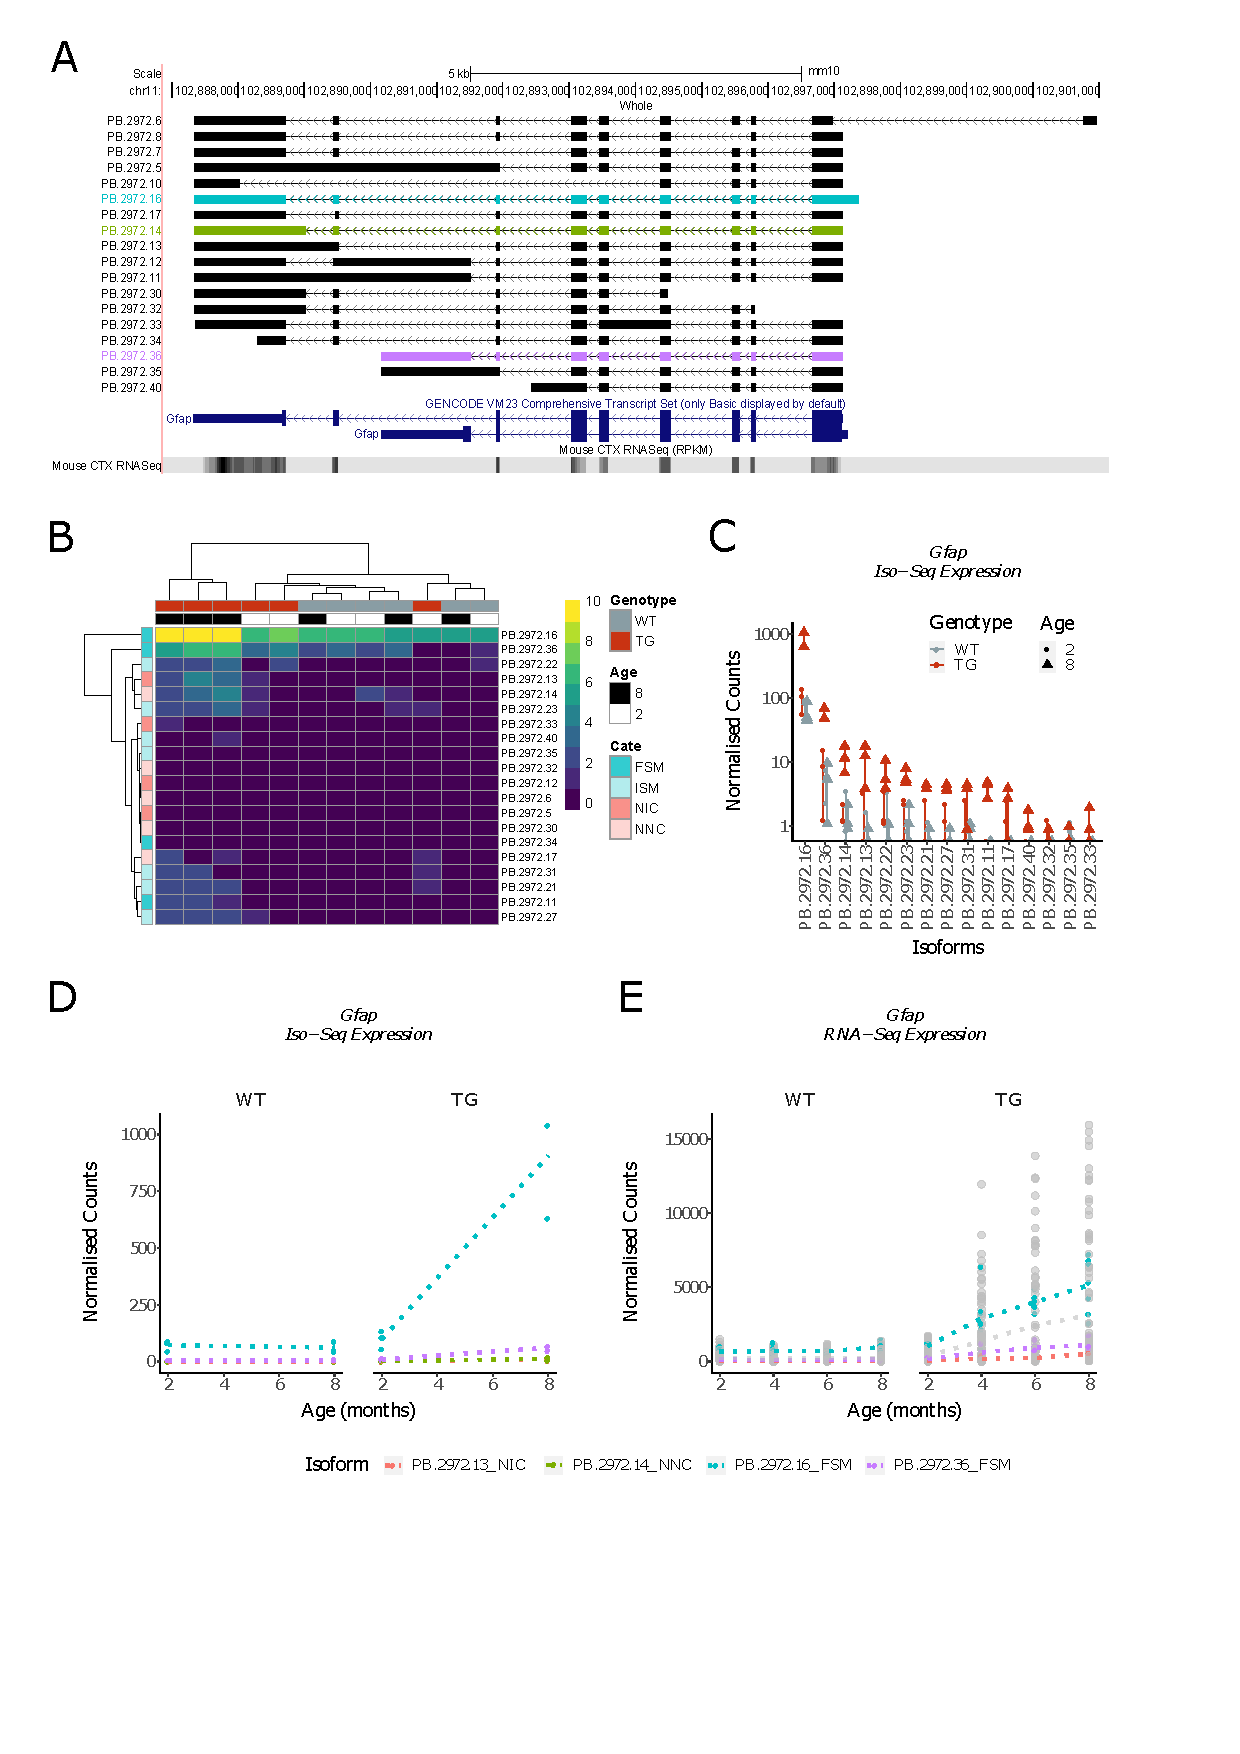
\includegraphics[page=1,trim={0.5cm 4.8cm 2cm 1cm}, scale = 0.85]{Figures/Ch5_DiffPlots.pdf}
	\captionsetup{width=0.95\textwidth}
	\caption[Differential \textit{Gfap} transcript expression in rTg4510 mice]%
	{\textbf{Significant up-regulation of the known isoform of \textit{Gfap} with progression of tau pathology in rTg4510 mice.} Shown are \textbf{(A)} UCSC genome browser tracks of isoforms annotated to \textit{Gfap}, \textbf{(B)} hierarchical clustering of \textit{Gfap}-associated isoforms by abundance (Iso-Seq FL read count, log2), \textbf{(C)} Normalised Iso-Seq FL read count of the top 15 most abundant isoforms, and \textbf{(D)} differentially expressed transcripts identified using normalised Iso-Seq read and \textbf{(E)} RNA-Seq read counts. Grey dots denote to differentially expressed transcripts identified using RNA-Seq but not Iso-Seq reads for quantification. FSM - Full Splice Match, ISM - Incomplete Splice Match, NIC - Novel In Catalogue, NNC - Novel Not in Catalogue. WT - Wild-type mice, TG - rTg4510 transgenic mice. Dotted lines represent the mean paths across age.} 
	\label{fig:DEI_gfap}
\end{figure}

\begin{figure}[!htp]
	\centering
	\includegraphics[page=2,trim={1.5cm 4.8cm 2cm 1cm}, scale = 0.85]{Figures/Ch5_DiffPlots.pdf}
	\captionsetup{width=0.95\textwidth}
	\caption[Differential \textit{C4b} transcript expression]%
	{\textbf{Significant up-regulation of the known isoform of \textit{C4b} with progression of tau pathology in rTg4510 mice.} Shown are \textbf{(A)} UCSC genome browser tracks of isoforms annotated to \textit{C4bp}, \textbf{(B)} hierarchical clustering of \textit{C4b}-associated isoforms by abundance (Iso-Seq FL read count, log2), \textbf{(C)} Normalised Iso-Seq FL read count of the top 15 most abundant isoforms, and \textbf{(D)} differentially expressed transcripts identified using normalised Iso-Seq read and \textbf{(E)} RNA-Seq read counts. Grey dots denote to differentially expressed transcripts identified using RNA-Seq but not Iso-Seq reads for quantification. FSM - Full Splice Match, ISM - Incomplete Splice Match, NIC - Novel In Catalogue, NNC - Novel Not in Catalogue. WT - Wild-type mice, TG - rTg4510 transgenic mice. Dotted lines represent the mean paths across age.}   
	\label{fig:DEI_c4b}
\end{figure}

\clearpage
\subsection{rTg4510 mice were characterised by the differential expression of transcripts of genes implicated in AD}
\label{ch5: diffisoexp}
The list of transcripts progressively altered in rTg4510 transgenic mice were annotated to genes previously implicated in AD development and pathology (\cref{tab:DEI_trans}). This included: i) Padi2-201 (ENSMUST00000030765.6) annotated to \textit{Padi2}/\textit{Pad2} (\cref{fig:Padi2}), which encodes for an enzyme that is abnormally activated in astrocytes from AD patients \cite{A2005}, ii) H2-D1-202 (ENSMUST00000172785.7) annotated to \textit{H2-D1} (\cref{fig:H2D1}), which encodes for major histocompatibility complex (MHC) class 1, an immune-related gene that is also up-regulated in microglia isolated from a neurodegenerative mouse model with AD-like phenotypes\cite{Mathys2017}, iii) Gatm-201 (ENSMUST00000028624.8) annotated to \textit{Gatm} (\cref{fig:Gatm}), encoding a mitochondrial protein recently revealed as a key AD protein signature \cite{Wang2020}, and iv) Ctsd-202 (ENSMUST00000151120.8) annotated to \textit{Ctsd} (\cref{fig:Ctsd}), encoding Cathepsin D, a lysosomal protease involved in A$\beta$ \cite{JR1996} and tau \cite{A1997} degradation, and a key regulator of A$\beta$\textsubscript{42/40} ratio\cite{Suire2020}, among others. Drawing parallels to \textit{Gfap} and \textit{C4b}, these genes were characterised by a dominant known isoform that was significantly up-regulated with progressive tau pathology, which was validated using RNA-Seq reads mapped to our improved Iso-Seq-derived transcriptome annotation. 


\begin{landscape}
\begin{table}[]
	\centering
	\setlength\tabcolsep{5.5pt} %reduced margin size in table
	\captionsetup{width=1.45\textwidth}
	\caption[Differentially expressed transcripts associated with rTg4510 genotype]%
	{\textbf{Differentially expressed transcripts associated with rTg4510 genotype.} Tabulated are the top-ranked differentially expressed transcripts between wild-type and rTg4510 transgenic mice using \textit{maSigPro}. Iso-Seq reads were used for both annotation and quantification.}
	\begin{threeparttable}
	\begin{tabular}{@{}cccccccccc@{}}
		\toprule
		\multirow{2}{*}{Rank\tnote{a}} &
		\multirow{2}{*}{Gene} &
		\multirow{2}{*}{Isoform} &
		\multirow{2}{*}{Isoform ID} &
		\multirow{2}{*}{FDR\tnote{b}} &
		\multirow{2}{*}{\begin{tabular}[c]{@{}c@{}}log\textsubscript{2} FC\textsubscript{genotype}\tnote{c}\end{tabular}} &
		\multicolumn{2}{c}{\begin{tabular}[c]{@{}c@{}}Mean WT \\ transcript expression\end{tabular}} &
		\multicolumn{2}{c}{\begin{tabular}[c]{@{}c@{}}Mean TG\\  transcript expression\end{tabular}} \\ \cmidrule(l){7-10} 
		&                 &                       &            &            &       & 2 months & 8 months & 2 months & 8 months \\ \midrule
		1   & \textit{Ubqln1} & ENSMUST00000058735.11 & PB.4255.13 & 7.43E-42   & 0.96  & 0.969 & 33.9  & 43.4  & 22.8  \\
		2   & \textit{C4b}    & ENSMUST00000069507.8  & PB.7004.8  & 5.9E-40    & 0.942 & 4.41  & 3.49  & 1.78  & 3.86  \\
		3   & \textit{Gfap}   & ENSMUST00000077902.5  & PB.2972.16 & 1.11E-35   & 0.933 & 3.19  & 72.3  & 60.9  & 99    \\
		4   & \textit{Tgfbr1} & ENSMUST00000007757.14 & PB.10959.1 & 1.09E-19   & 0.841 & 3.16  & 0.66  & 1.31  & 1.21  \\
		5   & \textit{Cd34}   & ENSMUST00000016638.7  & PB.1036.2  & 8.43E-18   & 0.894 & 1.99  & 1.31  & 5.4   & 2.71  \\
		29  & \textit{Padi2}  & ENSMUST00000030765.6  & PB.11607.2 & 5.2E-11    & 0.792 & 2.13  & 22.6  & 24.3  & 26.7  \\
		76  & \textit{H2-D1}  & ENSMUST00000172785.7  & PB.7039.1  & 8.47E-08   & 0.697 & 1.5   & 30.6  & 28.1  & 40.3  \\
		79  & \textit{Gatm}   & ENSMUST00000028624.8  & PB.9298.1  & 9.79E-08   & 0.738 & 0.869 & 29.1  & 34.5  & 34.6  \\
		175 & \textit{Ctsd}   & ENSMUST00000151120.8  & PB.15108.6 & 0.00000592 & 0.598 & 1.03  & 89.7  & 91.8  & 127   \\ \bottomrule
	\end{tabular}
	\begin{tablenotes}
		\footnotesize
		\item[a] The order of differentially expressed transcripts (n = 886) by FDR
		\item[b] False discovery rate
		\item[c] log\textsubscript{2} fold change of TG aged 8 months vs WT aged 8 months
	\end{tablenotes}
	\end{threeparttable}
	\label{tab:DEI_trans}
\end{table}
\end{landscape}

\begin{landscape}
	\begin{figure}[!htp]
		\centering
		\includegraphics[page=4,trim={1.5cm 3.5cm 2cm 1cm}, scale = 0.85]{Figures/Ch5_DiffPlots_Landscape.pdf}
		\captionsetup{width=1.5\textwidth}
		\caption[Differential \textit{Padi2} transcript expression]%
		{\textbf{Significant up-regulation of \textit{Padi2-201} with progression of tau pathology in rTg4510 mice.} Shown are \textbf{(A)} UCSC genome browser tracks of isoforms annotated to \textit{Padi2}, \textbf{(B)} hierarchical clustering of \textit{Padi2}-associated isoforms by abundance (Iso-Seq FL read count, log2), \textbf{(C)} differentially expressed transcript (Padi2-201, ENSMUST00000030765.6, PB.11607.2) identified using normalised Iso-Seq read and \textbf{(E)} RNA-Seq read counts. Grey dots denote to differentially expressed transcripts identified using RNA-Seq but not Iso-Seq reads for quantification. Dotted lines represent the mean paths across age.}   
		\label{fig:Padi2}
	\end{figure}	
\end{landscape}

\begin{landscape}
	\begin{figure}[!htp]
		\centering
		\includegraphics[page=2,trim={1.5cm 3.5cm 2cm 1cm}, scale = 0.85]{Figures/Ch5_DiffPlots_Landscape.pdf}
		\captionsetup{width=1.5\textwidth}
		\caption[Differential \textit{H2-D1} transcript expression]%
		{\textbf{Significant up-regulation of \textit{H2-D1-202} with progression of tau pathology in rTg4510 mice.} Shown are \textbf{(A)} UCSC genome browser tracks of isoforms annotated to \textit{H2-D1}, \textbf{(B)} hierarchical clustering of \textit{H2-D1}-associated isoforms by abundance (Iso-Seq FL read count, log2), \textbf{(C)} differentially expressed transcript (H2-D1-202, ENSMUST00000172785.7, PB.7039.1) identified using normalised Iso-Seq read and \textbf{(E)} RNA-Seq read counts. Grey dots denote to differentially expressed transcripts identified using RNA-Seq but not Iso-Seq reads for quantification. Dotted lines represent the mean paths across age.}   
		\label{fig:H2D1}
	\end{figure}	
\end{landscape}

\begin{landscape}
	\begin{figure}[!htp]
		\centering
		\includegraphics[page=3,trim={1.5cm 3.5cm 2cm 1cm}, scale = 0.85]{Figures/Ch5_DiffPlots_Landscape.pdf}
		\captionsetup{width=1.5\textwidth}
		\caption[Differential \textit{Gatm} transcript expression]%
		{\textbf{Significant up-regulation of \textit{Gatm-201} with progressive tau pathology in rTg4510 mice.} Shown are \textbf{(A)} UCSC genome browser tracks of isoforms annotated to \textit{Gatm}, \textbf{(B)} hierarchical clustering of \textit{Gatm}-associated isoforms by abundance (Iso-Seq FL read count, log2), \textbf{(C)} differentially expressed transcript (Gatm-201, ENSMUST00000028624.8, PB.9298.1) identified using normalised Iso-Seq read and \textbf{(E)} RNA-Seq read counts. Grey dots denote to differentially expressed transcripts identified using RNA-Seq but not Iso-Seq reads for quantifications. Dotted lines represent the mean paths across age.}   
		\label{fig:Gatm}
	\end{figure}	
\end{landscape}

\begin{landscape}
	\begin{figure}[!htp]
		\centering
		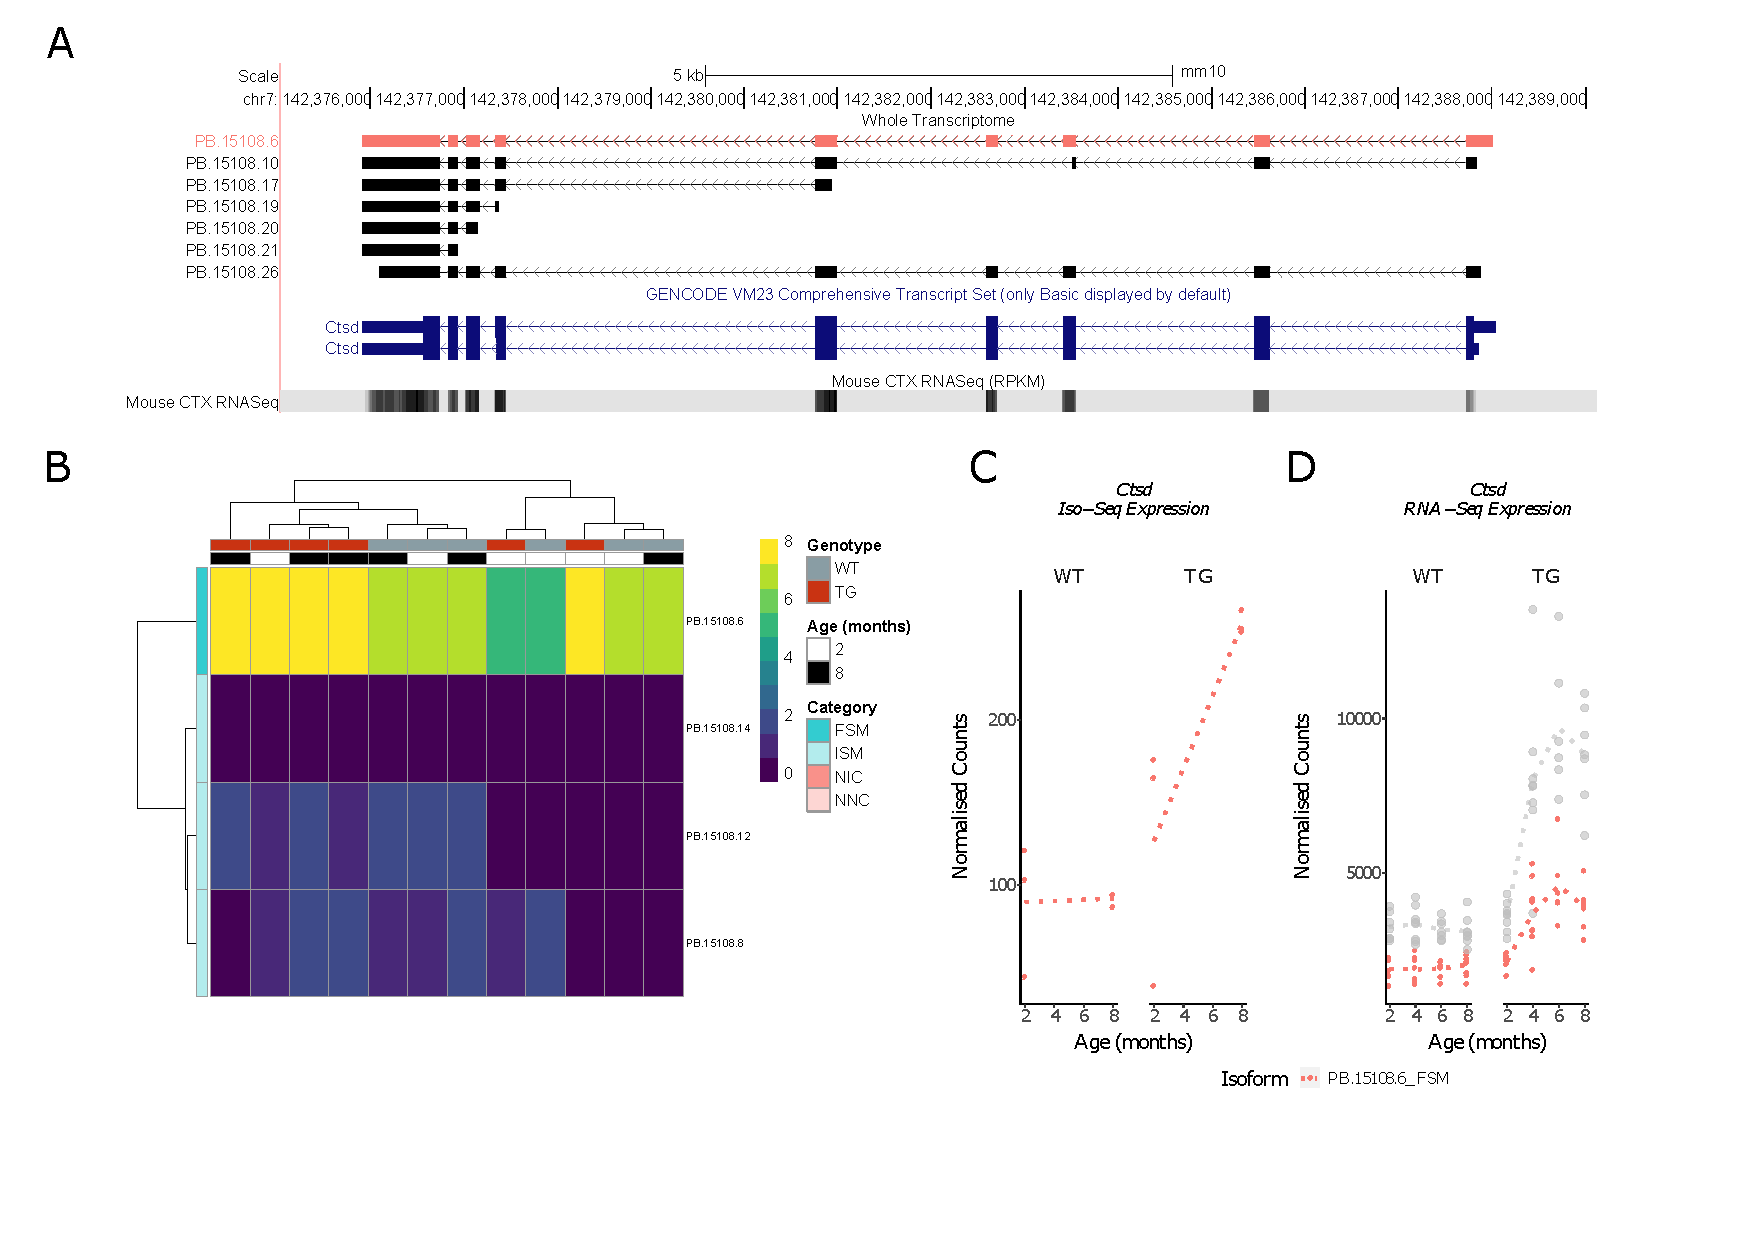
\includegraphics[page=1,trim={1.5cm 2.5cm 2cm 2cm}, scale = 0.85]{Figures/Ch5_DiffPlots_Landscape.pdf}
		\captionsetup{width=1.5\textwidth}
		\caption[Differential \textit{Ctsd} transcript expression]%
		{\textbf{Significant up-regulation of \textit{Ctsd-202} with progressive tau pathology in rTg4510 mice.} Shown are \textbf{(A)} UCSC genome browser tracks of isoforms annotated to \textit{Ctsd}, \textbf{(B)} hierarchical clustering of each \textit{Ctsd}-associated isoform based on abundance (Iso-Seq FL read count, log2), \textbf{(C)} differentially expressed transcript (Ctsd-202, ENSMUST00000151120.8, PB.15108.6) identified using normalised Iso-Seq read and \textbf{(E)} RNA-Seq read counts. Grey dots denote to differentially expressed transcripts identified from RNA-Seq but not Iso-Seq reads. Dotted lines represent the mean paths across age.}   
		\label{fig:Ctsd}
	\end{figure}	
\end{landscape}

Despite the demonstrated utility of using long reads for differential expression analysis, we found that the expression differences for the majority of Iso-Seq-identified differentially expressed transcripts (n = 545, 90.6\%) were not recapitulated with normalised RNA-Seq read counts. This included the top ranked transcript, Ubqln1-201 (ENSMUST00000058735.11, PB.4255.13) annotated to \textit{Ubqln1} and Cd34-201 (ENSMUST00000016638.7, PB.1036.2) annotated to \textit{Cd34} (\cref{tab:DEI_trans}). Although both transcripts were up-regulated with progressive tau pathology in rTg4510 mice using Iso-Seq FL read counts, no significant transcript expression differences were identified with normalised RNA-Seq read counts (\cref{fig:DEI_cd34_ubq}). We suspected that this could be partially due to the relatively low sensitivity of RNA-Seq reads to differentiate these almost-identical transcripts. Deeper examination of the Iso-Seq expression profiles, however, further revealed that while there was a difference in mean expression, there was also a large variance due to the relatively small number of samples profiled. We further noted that the majority of Iso-Seq-identified differentially expressed transcripts (n = 497 transcripts, 82.1\%) were very lowly-expressed (< 24 mean normalised FL reads, n = 12 samples). 

\begin{figure}[!htp]
	\centering
	\includegraphics[page=3,trim={1.5cm 3cm 2cm 1cm}, scale = 0.80]{Figures/Ch5_DiffPlots.pdf}
	\captionsetup{width=0.95\textwidth}
	\caption[Disparities in differential transcript expression analysis]%
	{\textbf{Disparities in differential transcript expression analysis.} Shown are \textbf{(A)} UCSC genome browser tracks of the isoforms annotated to \textit{Ubqln1}, with two isoforms identified as differentially expressed using \textbf{(B)} normalised Iso-Seq read counts but not using \textbf{(C)} RNA-Seq read counts for quantification. \textbf{(D)} UCSC genome browser tracks of isoforms annotated to \textit{Cd34}, \textbf{(E)} \textit{Cd34} Iso-Seq transcript expression profile and \textbf{(F)} \textit{Cd34} RNA-Seq transcript expression profile are also shown. The colours between the tracks and scatter plots refer to the respective Iso-Seq-identified differentially expressed transcript.
	}   
	\label{fig:DEI_cd34_ubq}
\end{figure}

\clearpage
\subsection{Hybrid approach identifies tau-pathology associated differential transcript usage with major isoform switching events}
Further complexity in transcriptional regulation is reflected in the fact that the expression of a gene may remain constant between conditions, but the \textit{relative} expression of individual isoforms (and thus isoform \textit{proportions}) may differ; this phenomenon is known as differential transcript usage (DTU) and is described in detail in \cref{intro:dtu}. We therefore assessed whether the relative isoform abundance for each gene altered with rTg4510 genotype and/or age, and whether there was switching of the dominant major (highest expressed) isoform between experimental groups (major isoform switching). 

Using Iso-Seq reads, we were not able to identify genes with differential transcript usage, likely reflecting the relatively low sequencing coverage and small sample size of our Iso-Seq experiments. In contrast, we identified 671 DTU genes (\cref{tab:DIU_DEA_nums}) when using normalised RNA-Seq read counts aligned to our Iso-Seq-derived transcriptome annotation (using the hybrid approach described in \cref{sec: gene_isoform_quant_explained}). Strikingly, the majority of these genes (n = 519, 77.3\%), while characterised by a change in isoform proportions, were not differentially expressed at the gene level between WT and TG mice. We further identified 61 genes that were not differentially expressed but were identified with both DTU and major isoform switching. This indicates that a significant degree of post-transcriptional regulation was independent of gene expression regulation. These genes (n = 580) were enriched as targets for a number of transcription factors (listed in \cref{tab: df_enrichr}), particularly TAF1 (adjusted \textit{P} = 1.10 x 10\textsuperscript{-6}, odds ratio = 1.77), which is a key component of the pre-initiation complex that initiates RNA polymerase II transcription\cite{Bieniossek2013}. 

\vspace{0.2cm}
\begin{table}[!htp]
	\centering
	\captionsetup{width=0.95\textwidth,singlelinecheck=off}
	\setlength\tabcolsep{6pt} %reduced margin size in table
	\caption[Summary of differential expression and splicing analyses]%
	{\textbf{Summary of differential expression and splicing analyses.} A summary of the number of genes identified as differentially expressed, and characterised with differential transcript usage and major isoform switching. Expression was determined using normalised RNA-Seq counts after alignment to the Iso-Seq-derived transcriptome.}
	\begin{tabularx}{0.92\textwidth}{cccc}
		\toprule
		\multicolumn{3}{c}{Conditions}                                                                                                                                                                                       & \multirow{2}{*}{Number of genes} \\ \cmidrule(r){1-3}
		\begin{tabular}[c]{@{}c@{}}Differential gene\\  expression\end{tabular} & \begin{tabular}[c]{@{}c@{}}Differential transcript \\ usage\end{tabular} & \begin{tabular}[c]{@{}c@{}}Major isoform\\  switching\end{tabular} &                                  \\ \midrule
		\checkmark  & \checkmark          & \checkmark                                                                & 16                               \\
		\checkmark                                                                      & \checkmark                                                                    & x                                                                  & 75                               \\
		x                                                                       & \checkmark                                                                    & \checkmark                                                                 & 61                               \\
		x                                                                       & \checkmark                                                                    & x                                                                  & 519                              \\ \midrule
		\multicolumn{3}{c}{Total number of genes}                                                                                                                                                                            & 671                              \\ \bottomrule
	\end{tabularx}
	\label{tab:DIU_DEA_nums}
\end{table}


\begin{table}[]
	\centering
	\captionsetup{width=0.95\textwidth,singlelinecheck=off}
	\caption[Transcription factor terms for differentially spliced genes]%
	{\textbf{Transcription factor terms for differentially spliced genes.} Tabulated is a list of the top 10 transcription factor terms (“ENCODE and ChEA Consensus TFs from ChIP-X”) for genes (n = 580) identified with differential isoform usage but no differential gene expression. Gene ontology analysis was performing using \textit{Enrichr}.}
	\label{tab: df_enrichr}
	\begin{tabular}{@{}ccc@{}}
		\toprule
		Term   & Adjusted \textit{P} & Odds ratio \\ \midrule
		TAF1   & 1.10 x 10\textsuperscript{-6}         & 1.771      \\
		MAX    & 5.78 x 10\textsuperscript{-6}         & 1.866      \\
		UBTF   & 7.76 x 10\textsuperscript{-5}          & 1.843      \\
		YY1    & 9.44 x 10\textsuperscript{-5}          & 1.645      \\
		RCOR1  & 1.68 x 10\textsuperscript{-4}         & 2.219      \\
		RUNX1  & 3.10 x 10\textsuperscript{-4}         & 1.834      \\
		BRCA1  & 3.10 x 10\textsuperscript{-4}         & 1.544      \\
		E2F1   & 3.10 x 10\textsuperscript{-4}         & 2.021      \\
		SP2    & 1.28 x 10\textsuperscript{-3}          & 1.846      \\
		NFYA   & 1.72 x 10\textsuperscript{-3}          & 1.549      \\ \bottomrule
	\end{tabular}
\end{table}

The top gene characterised by a major isoform switch was \textit{Cisd3} (FDR = 3.26 x 10\textsuperscript{-26}, \cref{fig:DIU_Cisd3}\textbf{A}), a mitochondrial iron-sulphur domain-containing protein involved in regulating iron homeostasis essential for mitochondrial function\cite{Wiley2007}. While there was little difference in overall gene expression (\cref{fig:DIU_Cisd3}\textbf{B}), a major isoform switch was observed between rTg4510 genotype that was consistent across all ages (\cref{fig:DIU_Cisd3}\textbf{C-E}). The two known isoforms (Cisd3-201 and Cisd3-202) involved in this switch only differed at the 5' end by the presence of an intron retention (IR) event occurring between exons 1 and 2. ORF predictions revealed that this IR event generated a shortened reading frame, which could translate to a different N-terminal peptide sequence (\cref{fig:DIU_Cisd3}\textbf{A}). Cisd3-201 (ENSMUST00000107583.2, PB.2833.2), which contained this IR event, was up-regulated with progressive tau pathology, while Cisd3-202 (ENSMUST00000107584.7, PB.2833.1) was down-regulated.  

Another gene with significant DTU but no difference in gene expression was \textit{Shisa5} (FDR = 1.26 x 10\textsuperscript{-11}, \cref{fig:DIU_shisa5}\textbf{A}), a transmembrane that modulate both Wnt and FGF signalling by inhibiting their maturation and trafficking to the cell surface\cite{Yamamoto2005}. An example of the compensatory mechanism that is sometimes observed with differential transcript expression, we identified a gradual isoform shift associated with progressive tau pathology (\cref{fig:DIU_shisa5}\textbf{D,E}). The two isoforms of interest differed significantly in length due to the usage of an alternative promoter (\cref{fig:DIU_shisa5}\textbf{A}); the longer isoform (Shisa5-201, ENSMUST00000026737.11, PB.16934.2) spanned the full-length of the gene across all six exons, whereas the shorter isoform (Shisa5-203, ENSMUST00000154184.4, PB.16934.9) lacked the first three upstream exons but contained an alternative first exon. Unsurprisingly, ORF prediction revealed a significant disparity in the ORF length with the longer isoform containing the whole Shisa Pfam domain. While the shorter isoform was the dominant isoform in wild-type mice across all ages, we observed a down-regulation of this isoform coupled with an up-regulation of the longer transcript in rTg4510 TG mice (\cref{fig:DIU_shisa5}\textbf{C,D}), resulting in a zero net change in gene expression (\cref{fig:DIU_shisa5}\textbf{B}). 

In addition to identifying genes with DTU but no overall differences in gene expression, we also identified genes with evidence for altered gene expression accompanied with differential transcript expression and major isoform switching. This included \textit{Fblim1} (FDR = 1.87 x 10\textsuperscript{-13}, \cref{fig:DIU_fblim1}\textbf{A}) - a gene that encodes for a filamin-binding protein involved in actin filament assembly and cell adhesion\cite{Takafuta2003} - which was up-regulated with progressive tau pathology in rTg4510 transgenic mice. Drawing parallels to \textit{Gfap} and \textit{C4b}, increased \textit{Fblim1} gene expression was also primarily driven by one isoform (\cref{fig:DIU_fblim1}\textbf{B}). However, this isoform was the less abundant, minor known isoform, Fblim1-203 (ENSMUST00000105785.8, PB.11626.1) found in wild-type mice rather than the dominant known isoform, Fblim1-202 (ENSMUST00000105784.7, PB.11626.2) (\cref{fig:DIU_fblim1}\textbf{D,E}). Given that detection of Fblim1-203 was negligible in wild-type mice, a strong increase in this isoform paralleling tau accumulation resulted in a robust isoform switch (\cref{fig:DIU_fblim1}\textbf{C}). Characterisation of these two isoforms revealed that they only differed by the presence of an alternative first exon, with the reading frame being broadly similar (\cref{fig:DIU_fblim1}\textbf{A}). 

Finally, we identified a novel fusion gene (this phenomenon is described in \cref{ch4:fusion_trans}), \textit{Arpc4-Ttll3} that was characterised by altered transcript usage and major isoform switching (FDR = 1.28 x 10\textsuperscript{-4}). Absent in the mouse reference genome annotation, three read-through transcripts (PB.13540.3, PB.13540.7, PB.13540.8) were annotated across the full-length of \textit{Arpc4} - which encodes one of the subunits of the Arp2/3 protein complex involved in actin polymerisation - and \textit{Ttll3} - which encodes the tubulin tyrosine ligase-like 1 (\cref{fig:DIU_Arpc4}\textbf{A}). The three transcripts differed by only 45bp at the first exon and the presence of exon 13 (exon 8 in \textit{Ttll3}) in PB.13540.7, which was skipped in the other two isoforms (\cref{fig:DIU_Arpc4}\textbf{A}). While there was no difference in overall gene expression (\cref{fig:DIU_Arpc4}\textbf{B}), we observed an isoform switch with PB.13540.7 up-regulation and  PB.13540.3 down-regulation in rTg4510 TG mice (\cref{fig:DIU_Arpc4}\textbf{C}), over time (\cref{fig:DIU_Arpc4}\textbf{D,E}). ORF predictions showed that skipping of exon 13 maintained the reading frame, although the predicted frame for all three transcripts only covered \textit{Ttll3} rather than spanning across both genes (\cref{fig:DIU_Arpc4}\textbf{A}).  

\newpage
\begin{figure}[!htp]
	\centering
	\includegraphics[page=4,trim={1.5cm 3.5cm 2cm 1cm}, scale = 0.80]{Figures/Ch5_DiffPlots.pdf}
	\captionsetup{width=0.95\textwidth}
	\caption[Differential \textit{Cisd3} transcript expression and usage]%
	{\textbf{Differential transcript expression and usage of \textit{Cisd3} with progression of tau pathology in rTg4510 mice.} Shown are \textbf{(A)} UCSC genome browser tracks of the isoforms annotated to \textit{Cisd3} with the two differentially expressed isoforms colour-coded and their respective predicted open reading frame (black), \textbf{(B)} \textit{Cisd3} gene expression, \textbf{(C)} proportion of isoform usage with rTg4510 genotype, independent of age, \textbf{(D)} \textit{Cisd3} transcript expression, and \textbf{(E)} proportion of isoform usage by age and genotype. Expression is determined from normalised RNA-Seq read counts after alignment to Iso-Seq-derived transcriptome.}    
	\label{fig:DIU_Cisd3}
\end{figure}

\begin{figure}[!htp]
	\centering
	\includegraphics[page=5,trim={1.5cm 1.5cm 2cm 1cm}, scale = 0.80]{Figures/Ch5_DiffPlots.pdf}
	\captionsetup{width=0.95\textwidth}
	\caption[Differential \textit{Shisa5} transcript expression and usage]%
	{\textbf{Differential transcript expression and usage of \textit{Shisa5} with progression of tau pathology in rTg4510 mice}: Shown are the \textbf{(A)} UCSC genome browser tracks of the isoforms annotated to \textit{Shisa5} with the two differentially expressed isoforms colour-coded, \textbf{(B)} \textit{Shisa5} gene expression, \textbf{(C)} proportion of isoform usage with rTg4510 genotype, independent of age, \textbf{(D)} \textit{Shisa5}-associated transcript expression and \textbf{(E)} proportion of isoform usage by age and genotype. Expression is determined from normalised RNA-Seq read counts after alignment to Iso-Seq-derived transcriptome.} 
	\label{fig:DIU_shisa5}
\end{figure}

\begin{figure}[!htp]
	\centering
	\includegraphics[page=6,trim={1.5cm 3cm 2cm 1cm}, scale = 0.80]{Figures/Ch5_DiffPlots.pdf}
	\captionsetup{width=0.95\textwidth}
	\caption[Differential \textit{Fblim1} transcript expression and usage]%
	{\textbf{Differential transcript expression and usage of \textit{Fblim1} with progression of tau pathology in rTg4510 mice}: Shown are the \textbf{(A)} UCSC genome browser tracks of the isoforms annotated to \textit{Fblim1} with the two differentially expressed isoforms colour-coded and their respective predicted open reading frame (black), \textbf{(B)} \textit{Fblim1} gene expression, \textbf{(C)} proportion of isoform usage with rTg4510 genotype, independent of age, \textbf{(D)} \textit{Fblim1}-associated transcript expression and \textbf{(E)} proportion of isoform usage by age and genotype. Expression is determined from normalised RNA-Seq read counts after alignment to Iso-Seq-derived transcriptome.} 
	\label{fig:DIU_fblim1}
\end{figure}

\begin{figure}[!htp]
	\centering
	\includegraphics[page=7,trim={1.5cm 1.5cm 2cm 1cm}, scale = 0.80]{Figures/Ch5_DiffPlots.pdf}
	\captionsetup{width=0.95\textwidth}
	\caption[Differential \textit{Arpc4-Ttll3} transcript expression and usage]%
	{\textbf{Differential transcript expression and usage of \textit{Arpc4-Ttll3} with progressive of tau pathology in rTg4510 mice.} Shown are \textbf{(A)} UCSC genome browser tracks of the three fusion transcripts annotated to \textit{Arpc4-Ttll3} with exon skipping (purple) and their respective predicted open reading frame (black), \textbf{(B)} \textit{Arpc4-Ttll3} gene expression, \textbf{(C)} proportion of isoform usage with rTg4510 genotype \textbf{(D)} expression of the fusion transcripts and \textbf{(E)} proportion of isoform usage by age and genotype. Expression is determined from normalised RNA-Seq read counts after alignment to Iso-Seq-derived transcriptome.} 
	\label{fig:DIU_Arpc4}
\end{figure}

\clearpage
\section{Discussion}

In this chapter, we leveraged the power of long-read sequencing to identify transcriptional and splicing differences associated with progressive tau pathology in a transgenic mouse model. To our knowledge, this represents the first comprehensive long-read sequencing dataset generated on a mouse model of tau pathology, facilitating the accurate interrogation of cortical expression alterations at the gene and transcript level. 

\subsection{Overview of results}
Demonstrating the dual utility of long reads for isoform annotation and quantification, we identified widespread gene expression differences paralleling the development of tau pathology in rTg4510 mice. At the gene-level, these results broadly recapitulated findings from our previous RNA-Seq study\cite{Castanho2020}, and implicate the role of transcriptional dysregulation in AD development. With the capacity to detect full-length transcripts, our study was further powered to identify robust genotype-associated differences in isoform expression. Notably, we found that the differential expression of two well-established AD-associated genes, \textit{Gfap} and \textit{C4b}, were primarily driven by the robust up-regulation of their dominant isoform. 

Although previous studies of gene expression have provided key insights into the molecular mechanisms driving AD pathogenesis\cite{Castanho2020,Salih2019,Annese2018,Magistri2015}, these studies fail to capture the dynamics in the expression of specific isoforms, particularly for genes where there are no overall gene expression differences. By complementing the improved isoform annotation provided by the long-read sequencing data with the deep sequencing depth achieved from short-read RNA-Seq data, we revealed a number of genes characterised with differential transcript usage (“isoform switching”) but no significant difference in global (gene-level) expression. Of note, these genes were involved in key pathways implicated in AD pathology, and included i) \textit{Shisa}, a modulator of the FGF and Wnt signalling pathways, which is essential for neuronal survival and is known to be suppressed in AD brains\cite{Jia2019}, ii) \textit{Cisd3}, a member of the same CDGSH domain-containing family as \textit{Cisd2}, which was recently identified as a promising new target in AD due to its neuroprotective role of the mitochondria against A$\beta$ accumulation\cite{Chen2020}, and iii) \textit{Arpc4}, which was recently found to co-aggregate with phosphorylated tau in NFTs extracted from AD patients\cite{Drummond2020} and in synaptosomes isolated from AD mouse models\cite{Li2020a}. Among these genes, we detected altered splicing and isoform switches with potential functional consequences.  
  
\subsection{Limitations}
\label{ch5: limitations}
Our results should be interpreted in the context of several limitations. Firstly, we performed long-read sequencing on a relatively small number of mouse samples. Although we found strongly consistent patterns of alternative splicing across biological replicates, we were unable to achieve the depth required to fully recapitulate the tau-associated transcriptional differences without relying on the deep RNA-Seq expression generated from matched samples. Notably, this hybrid approach still suffers from a degree of ambiguous alignment. We also observed that the relatively low sequencing depth afforded by global transcriptome profiling limits the power to perform differential splicing analysis. While we were able to detect differentially expressed isoforms using full-length read counts, we were unable to identify changes in isoform usage. This analysis requires reliable quantification of the relative proportion of isoforms, which is dependent on detecting all the isoforms, including the rare novel isoforms. Future work will aim to extend our analyses by sequencing larger numbers of samples and at a deeper sequencing depth. Profiling of the same samples using another long-read sequencing platform will also be useful to comprehensively investigate and validate the transcriptional variation associated with AD pathology. 

Secondly, our analyses were performed on bulk entorhinal cortex tissue, comprising a heterogeneous mix of neurons, oligodendrocytes and other glial cell-types. Despite compelling evidence from recent studies reporting cell- and disease-specific transcriptional signatures, we were unable to explore these differences in our datasets. This challenge can be addressed using a combined approach of single-cell sequencing and long-read sequencing, as shown in recent studies (reviewed in \cref{tab: longread_advancedstudies}) - however, this strategy is currently limited to achieve the depth required to detect reliable disease- and cell-specific splicing variations. Future work would build on recent methodological developments by our group that facilitate the purification of nuclei from different neural cell types prior to genomic profiling\cite{Stefprotocol}. 

Furthermore, while isoform expression was normalised for the library sequencing depth, our analyses did not account for differences in cellular composition between WT and rTg4510 TG mice. Given neuronal loss and astrogliosis are prominent hallmarks of AD pathogenesis, we were unable to discern whether transcriptional variations (i.e. up-regulation of astrocyte markers) are a direct consequence of AD-associated transcriptional regulation or a reflection of changes in cell composition. Future work should aim to use single-cell RNA-Seq data generated on similar samples (if available) or publicly-available single-cell datasets\cite{Joglekar2021} to infer cell type proportions in our bulk transcriptomic datasets. 

Finally, we only profiled entorhinal cortex tissue from female mice in order to minimise heterogeneity in our analyses. While the entorhinal cortex is an invariant focus of studying AD pathogenesis, as one of the first regions of the brain to be affected, tissue-specific differences in splicing and isoform usage of AD-risk genes have been previously reported\cite{Monti2021}. A number of sex differences have also been reported, with female mice exhibiting earlier and more severe cognitive and behavioural impairments than transgenic male mice\cite{M2011}. Future work should cross-examine results from our study with transcriptional variation in other tissue types and male mice for a more comprehensive understanding of the development of tau pathology in the AD brain. 

\subsection{Conclusion}
In summary, our study revealed transcriptional and splicing differences in the entorhinal cortex associated with tau accumulation. Importantly, we identified changes in key isoforms that drive the altered expression of AD-associated genes, with evidence of isoform switching events that could have important functional consequences. Our results demonstrate the utility of long-read sequencing data for isoform-level analyses, facilitating the detection of splicing alterations underlying the development of AD pathology. 